%%%%%%%%%%%%%%%%%%%%%%%%%%%%%%%%%%%%%%%%%
% Masters/Doctoral Thesis 
% LaTeX Template
% Version 2.2 (21/11/15)
%
% This template has been downloaded from:
% http://www.LaTeXTemplates.com
%
% Version 2.x major modifications by:
% Vel (vel@latextemplates.com)
%
% This template is based on a template by:
% Steve Gunn (http://users.ecs.soton.ac.uk/srg/softwaretools/document/templates/)
% Sunil Patel (http://www.sunilpatel.co.uk/thesis-template/)
%
% Template license:
% CC BY-NC-SA 3.0 (http://creativecommons.org/licenses/by-nc-sa/3.0/)
%
%%%%%%%%%%%%%%%%%%%%%%%%%%%%%%%%%%%%%%%%%

%----------------------------------------------------------------------------------------
%	PACKAGES AND OTHER DOCUMENT CONFIGURATIONS
%----------------------------------------------------------------------------------------

\documentclass[
12pt, % The default document font size, options: 10pt, 11pt, 12pt
%oneside, % Two side (alternating margins) for binding by default, uncomment to switch to one side
english, % ngerman for German
onehalfspacing, % Single line spacing, alternatives: onehalfspacing or doublespacing
%draft, % Uncomment to enable draft mode (no pictures, no links, overfull hboxes indicated)
%nolistspacing, % If the document is onehalfspacing or doublespacing, uncomment this to set spacing in lists to single
%liststotoc, % Uncomment to add the list of figures/tables/etc to the table of contents
%toctotoc, % Uncomment to add the main table of contents to the table of contents
%parskip, % Uncomment to add space between paragraphs
%nohyperref, % Uncomment to not load the hyperref package
headsepline, % Uncomment to get a line under the header
]{MastersDoctoralThesis} % The class file specifying the document structure

\usepackage[utf8]{inputenc} % Required for inputting international characters
\usepackage[T1]{fontenc} % Output font encoding for international characters

\usepackage{lmodern} % Use the Palatino font by default

\usepackage[sorting=none,backend=biber,style=numeric,natbib=true]{biblatex} % User the bibtex backend with the authoryear citation style (which resembles APA)

\addbibresource{thesis.bib} % The filename of the bibliography

\usepackage[autostyle=true]{csquotes} % Required to generate language-dependent quotes in the bibliography

\usepackage{amssymb,amsmath,enumerate}
\usepackage{graphicx}                                                                                                                                 
\usepackage[font=small,hypcap]{caption}
\usepackage{subcaption}
\usepackage{algorithm}% http://ctan.org/pkg/algorithms
\usepackage{algpseudocode}% http://ctan.org/pkg/algorithmicx
\usepackage{pdflscape}
\usepackage{amsmath,amsthm}

\newtheorem{definition}{Definition}
\newtheorem{theorem}{Theorem}
%----------------------------------------------------------------------------------------
%	MARGIN SETTINGS
%----------------------------------------------------------------------------------------

\geometry{
	paper=a4paper, % Change to letterpaper for US letter
	inner=1.5cm, % Inner margin
	outer=2.8cm, % Outer margin
	bindingoffset=2cm, % Binding offset
	top=1.5cm, % Top margin
	bottom=1.5cm, % Bottom margin
	%showframe,% show how the type block is set on the page
}

%----------------------------------------------------------------------------------------
%	THESIS INFORMATION
%----------------------------------------------------------------------------------------

\thesistitle{A New Methodology For Combining Graph Kernels} % Your thesis title, this is used in the title and abstract, print it elsewhere with \ttitle
\supervisor{Prof. Alessandro \textsc{Sperduti}} % Your supervisor's name, this is used in the title page, print it elsewhere with \supname
\cosupervisor{Dott. Nicol\`o \textsc{Navarin}} % Your supervisor's name, this is used in the title page, print it elsewhere with \supname
\examiner{} % Your examiner's name, this is not currently used anywhere in the template, print it elsewhere with \examname
\degree{Laurea Magistrale in Informatica} % Your degree name, this is used in the title page and abstract, print it elsewhere with \degreename
\author{Carlo Maria \textsc{Massimo}} % Your name, this is used in the title page and abstract, print it elsewhere with \authorname
\addresses{} % Your address, this is not currently used anywhere in the template, print it elsewhere with \addressname

\subject{Computer Science} % Your subject area, this is not currently used anywhere in the template, print it elsewhere with \subjectname
\keywords{} % Keywords for your thesis, this is not currently used anywhere in the template, print it elsewhere with \keywordnames
\university{Universit\`a degli Studi di Padova} % Your university's name and URL, this is used in the title page and abstract, print it elsewhere with \univname
\department{Dipartimento di Matematica} % Your department's name and URL, this is used in the title page and abstract, print it elsewhere with \deptname
\group{} % Your research group's name and URL, this is used in the title page, print it elsewhere with \groupname
\faculty{Facolt\`a di Informatica} % Your faculty's name and URL, this is used in the title page and abstract, print it elsewhere with \facname

\hypersetup{pdftitle=\ttitle} % Set the PDF's title to your title
\hypersetup{pdfauthor=\authorname} % Set the PDF's author to your name
\hypersetup{pdfkeywords=\keywordnames} % Set the PDF's keywords to your keywords

\begin{document}

\frontmatter % Use roman page numbering style (i, ii, iii, iv...) for the pre-content pages

\pagestyle{plain} % Default to the plain heading style until the thesis style is called for the body content

%----------------------------------------------------------------------------------------
%	TITLE PAGE
%----------------------------------------------------------------------------------------

\begin{titlepage}
\begin{center}

\begin{figure}
    \centering
    
\includegraphics[scale=2]{Figures/logounipd2}
\end{figure}

\textsc{\LARGE \univname}\\[1cm] % University name
\textsc{\large \deptname}\\[0.5cm] % Thesis type
 
\textsc{ Corso di Laurea Magistrale in Informatica}\\[0.5cm] % Thesis type
\textsc{\small Anno Accademico 2015-2016}\\[1cm] % Thesis type

\HRule \\[0.4cm] % Horizontal line
{\huge \bfseries A New Methodology For Combining Graph Kernels\par} % Thesis title
\vspace{0.4cm}
\HRule \\[1.5cm] % Horizontal line

\begin{minipage}[t]{0.4\textwidth}
\begin{flushleft} \large
\emph{Studente:}\\
\authorname\\1058513 % Author name - remove the \href bracket to remove the link
\end{flushleft}
\end{minipage}
\begin{minipage}[t]{0.5\textwidth}
\begin{flushright} \large
\emph{Relatore:} \\
\supname\\ % Supervisor name - remove the \href bracket to remove the link  
\emph{Co-relatore:} \\
\cosupname % Supervisor name - remove the \href bracket to remove the link  
\end{flushright}
\end{minipage}\\[3cm]

%{\large \today}\\[4cm] % Date
%\includegraphics{Logo} % University/department logo - uncomment to place it
 
\vfill
\end{center}
\end{titlepage}

\cleardoublepage

%----------------------------------------------------------------------------------------
%	QUOTATION PAGE
%----------------------------------------------------------------------------------------

%\vspace*{0.2\textheight}
%
%\noindent\enquote{\itshape 'OMG this is so meta I cant even}\bigbreak
%
%\hfill clojure

%----------------------------------------------------------------------------------------
%	ABSTRACT PAGE
%----------------------------------------------------------------------------------------

\begin{abstract}
\addchaptertocentry{\abstractname} % Add the abstract to the table of contents


Graph mining and particularly kernelized learning algorithms for graph-structured data
have seen a steady growth in popularity during the last decades. A number of improvements
over the existing graph kernels, have recently been proposed, further raising the performance limits.
The procedure to estimate the performances of these kernels in real applications
is still computationally demanding due to the essential process of hyper-parameter selection.
In this study we want to determine if it is possible to devise a method that can
substitute the commonly adopted procedures of kernel hyper-parameter selection,
avoiding it entirely while preserving the predictive performances of the method.

To assess the generality of the proposed methodology we analyse six
different kernels, namely we consider three graph kernels that have recently
been extended with contextual information and employ the contextualized and
non-contextualized version for each one.
The analyses are derived from commonly adopted real world bio-chemical datasets.

Empirical results show that the proposed methodology is faster than the 
baseline method when considering large scale kernel combination while always
maintaining comparable and in some cases superior performances.
\end{abstract}

%----------------------------------------------------------------------------------------
%	ACKNOWLEDGEMENTS
%----------------------------------------------------------------------------------------

%\begin{acknowledgements}
%\addchaptertocentry{\acknowledgementname} % Add the acknowledgements to the table of contents
%
%I would deeply and sincerely like to thank\dots
%
%
%\end{acknowledgements}

%----------------------------------------------------------------------------------------
%	LIST OF CONTENTS/FIGURES/TABLES PAGES
%----------------------------------------------------------------------------------------

\tableofcontents % Prints the main table of contents

\listoffigures % Prints the list of figures

\listoftables % Prints the list of tables

\listofalgorithms

%----------------------------------------------------------------------------------------
%	ABBREVIATIONS
%----------------------------------------------------------------------------------------

\begin{abbreviations}{ll} % Include a list of abbreviations (a table of two columns)

\textbf{MKL} & \textbf{M}ultiple \textbf{K}ernel \textbf{L}earning\\
\textbf{ST} & \textbf{S}ub \textbf{T}ree\\
\textbf{WL} & \textbf{W}eisfeiler-\textbf{L}ehman\\
\textbf{ODD} & \textbf{O}rdered \textbf{D}AG \textbf{D}ecomposition\\
\textbf{TCK} & \textbf{T}ree \textbf{C}ontext \textbf{K}ernel\\
\textbf{AUROC} & \textbf{A}rea \textbf{U}nder the \textbf{R}eceiver \textbf{O}perator \textbf{C}urve\\

\end{abbreviations}

%----------------------------------------------------------------------------------------
%	PHYSICAL CONSTANTS/OTHER DEFINITIONS
%----------------------------------------------------------------------------------------

%\begin{constants}{lr@{${}={}$}l} % The list of physical constants is a three column table

% The \SI{}{} command is provided by the siunitx package, see its documentation for instructions on how to use it

%	Speed of Light & $c_{0}$ & \SI{2.99792458e8}{\meter\per\second} (exact)\\
%Constant Name & $Symbol$ & $Constant Value$ with units\\

%\end{constants}

%----------------------------------------------------------------------------------------
%	SYMBOLS
%----------------------------------------------------------------------------------------

%\begin{symbols}{lll} % Include a list of Symbols (a three column table)
%
%$\phi$ & features mapping function \\
%%Symbol & Name & Unit \\
%
%%\addlinespace % Gap to separate the Roman symbols from the Greek
%
%\end{symbols}

%----------------------------------------------------------------------------------------
%	DEDICATION
%----------------------------------------------------------------------------------------

%\dedicatory{To my parents, to whom I owe this achievement.}
%{To my friends that, even though a great distance is between us most of the time,
%managed to be of invaluable help and motivation.} 
%{To you, that made me believe in my dreams again.}

%----------------------------------------------------------------------------------------
%	THESIS CONTENT - CHAPTERS
%----------------------------------------------------------------------------------------

\mainmatter % Begin numeric (1,2,3...) page numbering

\pagestyle{thesis} % Return the page headers back to the "thesis" style

% Include the chapters of the thesis as separate files from the Chapters folder
% Uncomment the lines as you write the chapters

% Chapter 1

\chapter{Introduction} % Main chapter title
\label{Chapter1} % For referencing the chapter elsewhere, use \ref{Chapter1} 

This chapter presents a brief overview of the present thesis.
First we introduce some basic concept about data and knowledge along with some examples,
then the main contribution is explained with some more in-depth discussion,
followed by the document outline.

\section{Relationship between data and knowledge}

The current amount of digital data produced daily is estimated to be in the realm of 
ZettaBytes ($1~ZB = 10^{12}~GB$) \cite{idc}.
Of this amount, only a small fraction sees actual processing and interpretation,
mainly because while the flow of information is steady, the available resources
devoted to the task are often limited \cite{idc}.
Moreover in some cases the rapidity at which a meaningful interpretation of the 
raw data has to be produced is critical.
Hence, just the plain fact of owning the data does not imply that some useful 
information pattern can be derived from it; in fact the whole discipline of \emph{Data Mining}
was born with the intent of derive \emph{knowledge} that ``we don't know we don't know''.

Most of data mining techniques draw from a variety of other fields like Statistics,
Computer Science, Information Theory and Mathematics just to mention a few.
This discipline rests its theoretical foundation upon the field of \emph{Machine Learning},
the discipline that studies algorithms and techniques that allows a machine
to learn a concept (or an approximation of it) from a set of examples.
These algorithms start from limited evidence and try to build up a general model
by refining an initial \emph{hypothesis}.
Machine Learning is mostly useful when either an exact solution to a very
difficult problem is computationally infeasible or the problem specification
is rather vague or not unambiguously defined, leaving to the algorithm the burden
of exploration.

One of the pivotal concepts of this field is data \emph{representation}.
For the most part, data is collected and stored in unstructured form, e.g. vectors,
and a lot of machine learning techniques are tailored to this representation.
In the last decades some approaches tried to address those problems whose data cannot
be represented in vectorial form or whose representation in this form would cause
information loss.
%----------------------------------------------------------------------------------------

\section{Why structured data}
\label{sec:why}
% ci sono un sacco di dati strutturati
% c'e` la necessita` di applicare machine learning
% se li rappresentiamo come vettori non va bene perche` si perde struttura e piu`
% cresce il mapping piu` trattarlo diventa difficile.

The increasing amount of available structured data has made it necessary to develop
machine learning methods that can effectively deal with it.
More specifically some work has been done to devise methods that could learn
directly from graphs, a very useful kind of \emph{structured data} that sees many
important real-world applications nowadays, encompassing the fields of Computational
Biology, Computer Vision and Natural Language Processing.
For these applications it is natural to collect data that carries an inherent
amount of information concerning its structure.
That is, some data is naturally structured, e.g. molecular graphs or a sentence parse tree,
and represent it in vectorial form will inevitably cause a loss of information about
its structure.
Moreover, adding structural information to a vectorial representation
makes it more complex and consequently more difficult to work with.

Graphs are a structured data form that can represent a great deal of different
information depending on the domain of application.
Graphs have multiple levels of information semantics and each level can have
different connotations, e.g. consider the set of edges, they can represent
different notions of link between two nodes while maintaining the same
representation.
Beside edges, that express a kind of local ``relationship''
information among the nodes, we have information stored at the node level in the
labels, where some qualitative or quantitative data may be present.
At a higher level we have topological information, which can be
viewed like an extended relationship level, and finally the information that can
be derived by looking at the shape of the graph such as notions
of connectivity, density etc.

\subsubsection{Examples}
\label{subsubsec:examples}

Chemical compounds are naturally represented by their molecule; a simple graph
representation of a molecule is given in Figure \ref{fig:chem}.
Most of the benchmark datasets employed in this study contain chemical compounds
represented in a similar way.

\begin{figure}[ht]
    \centering
    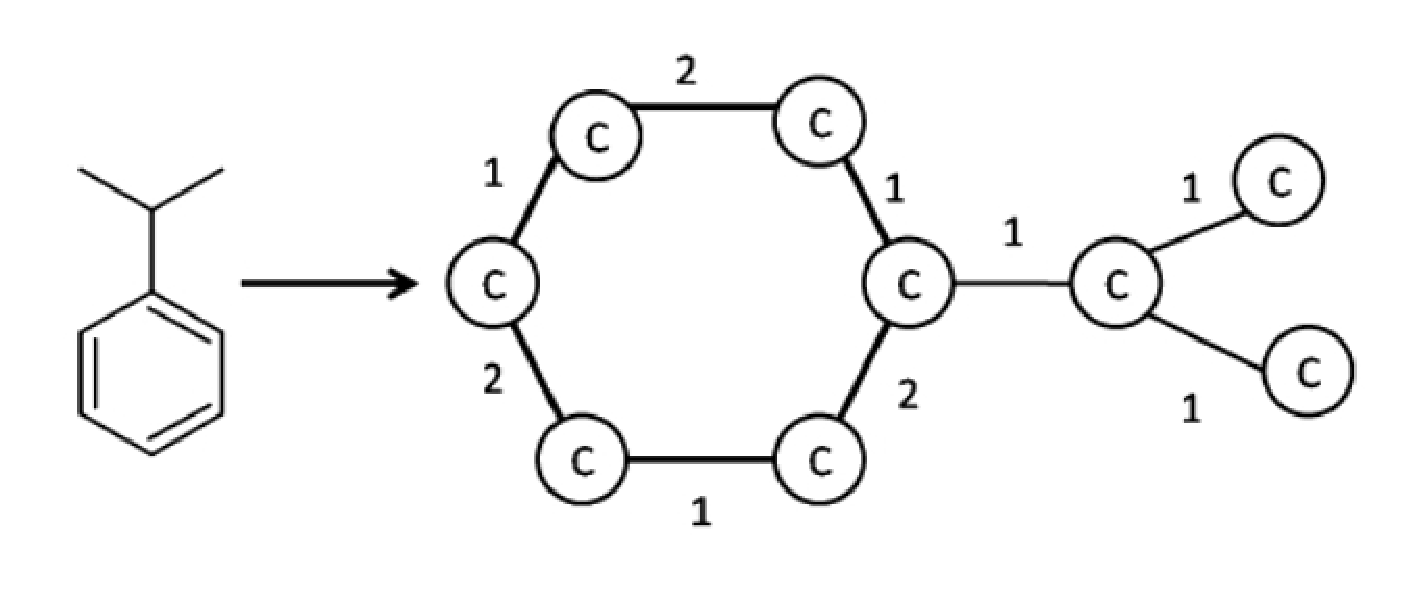
\includegraphics[scale=0.4]{Figures/chcomp}
    \caption{A molecule representation for a chemical compound and its representation
    as a graph; the nodes represent the atoms, the edges represent the chemical bounds and
    are labeled accordingly.}
    \label{fig:chem}
\end{figure}

Graph structured data has proven useful in the classification of non-coding RNA
molecules, modeled as shown in Figure \ref{fig:bio} \cite{nnavarin, conf/psb/KarklinMH05},

\begin{figure}[ht]
    \centering
    \begin{subfigure}{.4\textwidth}
        \centering
        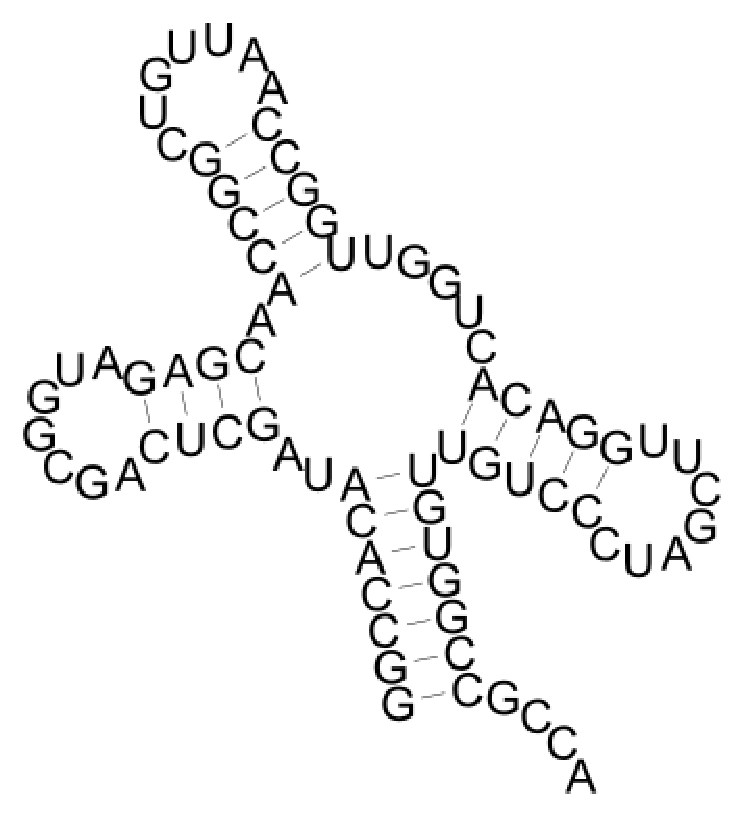
\includegraphics[width=\linewidth]{Figures/rna}
        \label{fig:rna}
        \caption{}
    \end{subfigure}
    \begin{subfigure}{.4\textwidth}
        \centering
        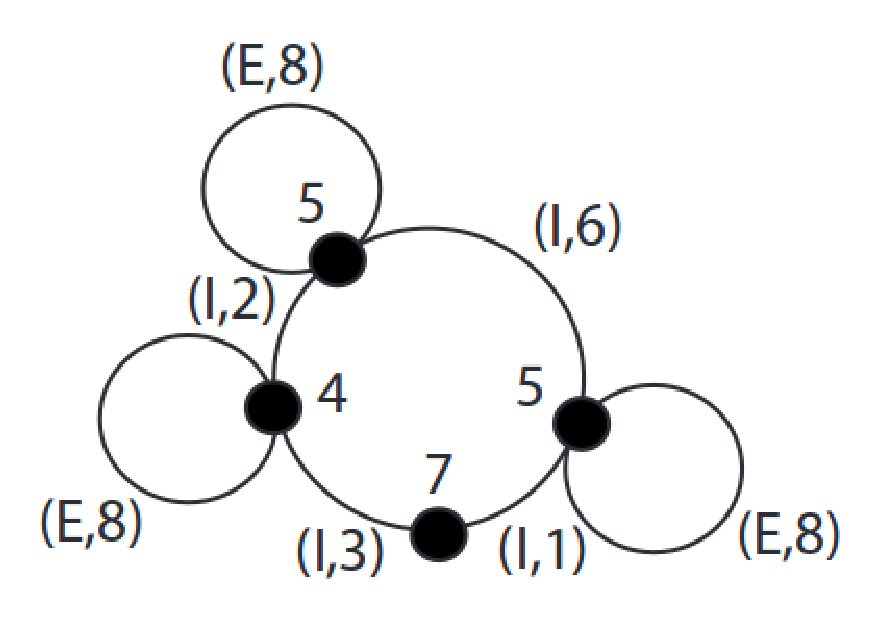
\includegraphics[width=\linewidth]{Figures/ldgrna}
        \label{fig:ldg}
        \caption{}
    \end{subfigure}
    \caption{a) RNA molecule graph representation and b) the same molecule represented
        as a labeled dual graph \cite{conf/psb/KarklinMH05}.}
    \label{fig:bio}
\end{figure}

Natural Language Processing is another field where graph representation is often used
as the basis for elaborate meaning extraction, as is the case for building opinion
lexicon from users review \cite{10.1371/journal.pone.0079294}, see Figure \ref{fig:wordrel}.

\begin{figure}[ht]
    \centering
    \includegraphics[width=.6\linewidth]{Figures/wordrel}
    \caption{Example of graph representation of words relationships in a multilingual
    context \cite{10.1371/journal.pone.0079294}.}
    \label{fig:wordrel}
\end{figure}

In Computer Vision a prominent application that uses graph representation is
the so-called scene understanding or scene modelling task, i.e. a scene is divided
into semantically meaningful areas which can be seen as nodes of a graph whose
edges are the adjacency relations between the areas \cite{journals/corr/abs-1108-4079},
an exemplification of this is given in Figure \ref{fig:scene}.

\begin{figure}[ht]
    \begin{subfigure}{.45\linewidth}
        \centering
        \includegraphics[width=\linewidth]{Figures/scene}
        \caption{}
        \label{fig:scene}
    \end{subfigure}
    \begin{subfigure}{.45\linewidth}
        \centering
        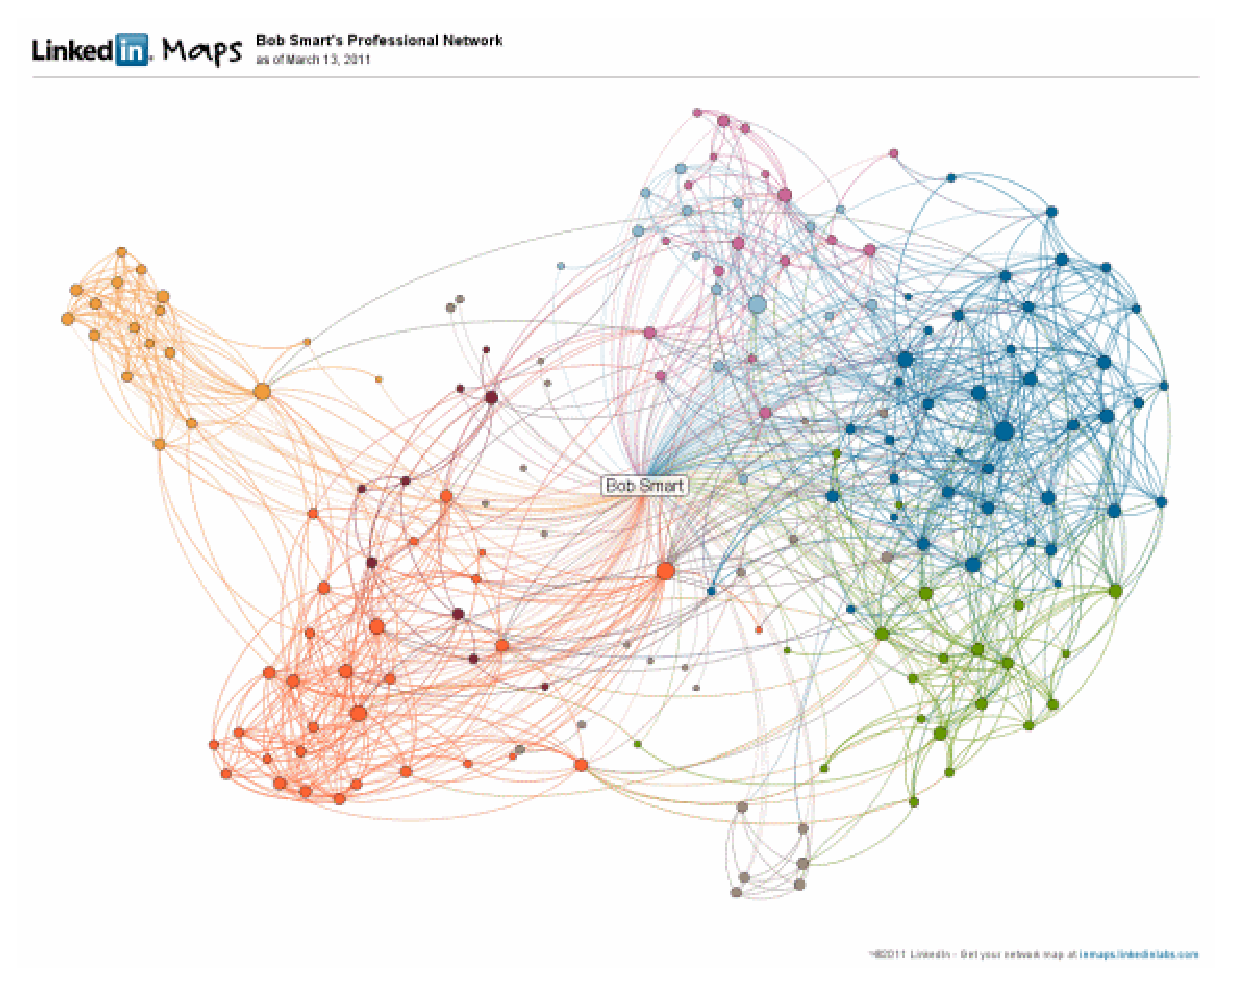
\includegraphics[width=\linewidth]{Figures/linkedin-social-maps}
        \caption{}
        \label{fig:network}
    \end{subfigure}
\caption{a) Scene understanding via graph decomposition in Computer Vision. b)
        LinkedIn's social maps show how a social network graph representation
        can quickly become very complex.}
\end{figure}

Finally, graphs deriving from the inherently structured organization of every social
network can lead to a large number of mining possibilities given the vast
amount of data available \cite{gundecha2012mining}.
Figure \ref{fig:network} shows an example of social network derived from a real-world
application.

%----------------------------------------------------------------------------------------

\section{Graph kernel learning}

Given the wealth of available data, how can we learn from graphs? A first \emph{structure-based}
approach consists in designing an \emph{ad-hoc} vectorial representation for the
particular kind of graphs being considered.
A major downside of this approach is that a renewed effort for the 
design of a new representation is needed every time a new type of data
is encountered.

Another way to address the problem of graph learning is to adapt the existing methods
to work directly on graphs, thus allowing the exploitation of the existing techniques.
Some recently proposed works \cite{DBLP:conf/sdm/MartinoNS12, NIPS2009_3813}
embed graph specific knowledge into well established \emph{kernel methods}
that, given the inherent decoupling between the data representation and the learning
algorithm that they provide (more on Section \ref{subsec:introkm}), represent a
more general approach.

This thesis focuses on these kernel methods, and their use on a binary classification
task in a supervised setting that is, a task in which the machine learning algorithm
has to separate (classify) two sets of already labelled samples (hence ``supervised'').
In the following sections we assume to be operating in this scenario.

\subsection{Kernel methods}
\label{subsec:introkm}

Kernel methods are a collection of techniques that rely on an implicit representation
of the data and a well defined measure of similarity between samples to perform
the learning task.
These methods have two main components: a domain specific function to compute the
samples similarity score, called \emph{kernel function}, and a general purpose
learning algorithm, often called \emph{kernel machine}, to combine the information provided by the
kernel function in order to separate the samples.

Kernel functions implicitly map examples in a high dimensional space, commonly
referred to as \emph{feature space}, and define the similarity score as a dot
product in this space.
Specific domain knowledge gets embedded in the learning process through the definition
of the kernel function that becomes the only interface between the data
and the learning algorithm.
The explicit representation of the feature space is never accessed by the algorithm
that refers to it only implicitly through the kernel function.
This is commonly known as the \emph{kernel trick} and the reason behind it is 
that computing the dot product for each pair of samples in a high dimensional space
would be infeasible but can be avoided thanks to the kernel function since they are
equivalent (Section \ref{subsec:kernelfunc}).

Kernel machines are learning algorithms that employ the similarity measures defined
by kernel functions to find a linear separator in a high dimensional feature space
since it is usually easier; once a separator has been found, it is mapped back
to the original input space from where the data was generated.
One of the most adopted methods is the Support Vector Machine (SVM) \cite{Cortes&Vapnik:1995}
which is a binary classifier that tries to find a separator that maximizes the \emph{margin}
between two sets of labelled samples that is, the distance between the separator and the
nearest sample of each class.
SVMs employ the samples pairwise distance as their similarity measure.

\subsection{Hyper-parameter selection}
\label{subsec:hyper1}

Most learning methods have parameters that need tuning, i.e. in order to achieve
good generalization performances each value has to be selected from a set of
possible choices according to a performance measure.
These parameters, often referred to also as \emph{hyper-parameters}, define a
\emph{parameter space} characterized by their number, and by the size and type
of their domains.
This space can be potentially infinite and it is usually highly non-convex, making
the search for a global optimum very hard, if any exists.

For this reason the selection procedure often involves a limited search on the parameter space
that is, a set of values for each parameter is fixed, possibly after a discretization,
and all the combinations are tested to find the best one.
However, in order to be useful the sampling on the parameter space needs to be adequate:
even with a heuristic approach the complexity of this search can still be daunting because
it depends on the number of parameters.

In the context of kernel learning hyper-parameters can be found on two levels:
parameters relative to the kernel function and parameters that belongs to the
kernel machine (solver).
The parameters of the former typically influence the feature space being generated,
directly affecting the expressiveness of the similarity measure, i.e. the ability
to discern between two different samples.
The parameters of the solver are usually employed as regularization factors,
as is the case for the SVM, where its only hyper-parameter is used to balance the trade-off between a good
(generalizing) separator and empirical error.
Once the solver has been chosen, the parameter space is determined by the kernel
hyper-parameters hence, the kernel choice can greatly affect the computational
performances of the whole approach.
Moreover, often the kernel has to be selected in a similar way, thus increasing the
computational burden even more.

\subsection{Validation procedures}
The learning process is composed of two main phases, the training phase and
the test phase.
Briefly, in the training phase a model is built trying to approximate a concept, its performances
are then assessed during the test phase.
Each phase employs a different set of data, training data and test data respectively,
that is sampled from the original dataset.
Hyper-parameter values can deeply affect these two phases, in particular
because they determine which hypotheses are selected by the learning algorithm.
There are two main factors that are influenced by the values selected for the
hyper-parameters.

On one hand we have \emph{overfitting}, which happens when the hypothesis
(model) returned by the training phase is able to correctly classify the training data
but performs poorly on new instances that get presented to it, i.e. the test data.
This can happen because the selected hyper-parameter values render the model so
complex that it fits to spurious properties of the training data.

On the other hand we have \emph{underfitting} which consists in the hypothesis skewing
in a direction that makes it unable to grasp the full complexity of the data resulting
in a high classification error even on the training data.
This can be due to the model being too simple because of the chosen parameter values. 

To find the optimal balance between these two factors, typically hyper-parameter
selection is performed employing a \emph{validation set}, that is a fixed subset of the
data left out from the training phase and used to validate the performances of a
model built according to a given set of values for the parameters.
In this case the validation set coincides with the test data.
To reduce the bias, i.e. the distortion, deriving from the fixed selection of
the validation set, a k-fold cross-validation technique is employed: the
data is split into $k$ subsets, $k-1$ become the training set while the last one
is used as the validation set; this procedure is repeated $k$ times, with the
validation set being a different one of the $k$ subsets during each iteration
(\emph{fold}).

This way the best performing model built according to a set of parameter values
is selected, which is equivalent to select the best set of parameter values.
This process is still prone to overfitting because, due to the way cross-validation
is performed, the final model gets trained and validated on the same
data.

\subsubsection{Nested cross-validation}
A remedy to the possible overfitting deriving from a cross-validation,
the so-called nested k-fold cross validation is employed.
This technique consists in two k-fold cross-validation nested one within the other.
In the outer loop the whole dataset is split in $k$ subset, one of which becomes the
\emph{test set}.
The remaining training data is then used to perform a regular k-fold cross-validation
whose selected model is trained again on the whole training set and finally evaluated
on the test set.
This technique ensures that the test set is completely left out from the training
process so that the performance estimation is independent from the training data.
The performances estimated on the $k$ obtained models are then averaged and represent
an unbiased performance estimate of the best performing model given the available data.

%\subsection{Proposed solution}
\section{Thesis contribution}
% more detail
% relevance
The task of estimating a model performance is essential in machine learning
but can become very onerous to perform, especially when employing a nested 10-fold
cross-validation technique, 10 being usually a reasonable value for $k$, which
increases the computational times a couple of orders of magnitude with respect
to a single training phase.
Moreover the size and shape of the (finite) parameter space considered while performing
hyper-parameter selection will directly impact on the overall time required to
obtain the desired results.

% problem
% kernel learning typically has a number of params to select
% graph kernel learning more so
% single kernel approach test each kernel ie function+params in isolation
% this can be a problem because kernel computation tends to be heavy.
% so a lot of kernels = a lot of time

Kernel learning methods needs to select the optimal values for a number of parameters
belonging both to the kernel function and to the kernel machine of choice.
Kernel function parameters shape the underlying feature space thus greatly affecting
the resulting kernel performances. Hence the number of values to select from has
to be sized in order to allow a good sampling.
With the standard approach each kernel, i.e. the combination of a kernel function
and a set of parameter values, has to be computed and tested individually and this can
further slow down hyper-parameter selection.
This is particularly true for graph kernel learning, since graph kernels are usually
computationally demanding (Section \ref{subsec:graphk}).

% sol

% intro mkl
A different approach, called \emph{multiple kernel learning} (MKL), has been
developed to allow the combination of different kernels into a single learning phase.
This family of methods typically tries to find the best (non) linear combination between the
given kernels, to increase the individual performances and implicitly perform the
kernel selection in a data driven way.
This approach has been developed with the initial aim to be employed with a small
number of independent and carefully designed kernels in order to beat simpler combination
such as the average.
Recently a second approach has been emphasized that is, combine a large set of possibly
weak kernels with the intended purpose of boosting the overall accuracy.
From the numerous implementations available in literature \cite{journals/jmlr/GonenA11},
we want to mention EasyMKL, a recently proposed state-of-the-art MKL implementation
\cite{aiolli2015easymkl} with a linear complexity bound w.r.t. the input size.
This algorithm is an \emph{optimization based} MKL implementation with a strong
theoretical background (Section \ref{subsec:easymkl}) and was selected to be part
of the this work.

In this study we propose a methodology to perform graph kernel learning avoiding
the process of kernel hyper-parameter selection, reducing the overall time
required to do the model performance estimation without significantly losing
predictive performances.
Employing EasyMKL combination capabilities from a different perspective, we
perform the learning task employing at once all the kernels that would have been
individually computed according to a kernel parameters grid (Section \ref{subsubsec:grid}).
Therefore we achieve a consistent reduction of the hyper-parameters to validate, since
eliminating all the kernel function parameters from the selection process, only those of the
kernel machine remain.

% results

The obtained results show on average a significant decrease in computational times across the
considered datasets while the predictive performances remain comparable when not
above the selected baseline methods.
Moreover, the proposed methodology can be generalized to consider multiple kernel functions.

With this approach the whole process of hyper-parameter selection has been streamlined and
lifted from the kernels to the learning machine, effectively eliminating the need to test each
kernel in isolation.

%----------------------------------------------------------------------------------------

\section{Thesis outline}
This document is organized as follows: in Chapter \ref{Chapter2} we delve into
the background details that are necessary to fully understand the proposed idea;
we cover the basics of machine learning and kernel methods and see some examples
of kernel combination techniques.
The main ideas behind this work are exposed in Chapter \ref{Chapter3} where we
discuss in detail our approach, the conceptual steps involved and the solutions
to the problems encountered.
Chapter \ref{Chapter4} covers the experimental part of the thesis, where we present
our results and finally in Chapter \ref{Chapter5} we draw conclusions and explain
how some ideas proposed here can be further explored.

%----------------------------------------------------------------------------------------

% vim: spell spelllang=en_gb
 % Introduction
% Chapter 2

\chapter{Background} % Main chapter title
This chapter covers in more detail the fundamental concepts needed to assure a
thorough comprehension of the topics discussed in the following chapters.
We start by giving a definition of machine learning, analysing the 
principal aspects of the general approach such as risk minimization and evaluation
strategy.
Then Section \ref{sec:kernel} deals with the theoretical foundations of the 
methods that are in the scope of this thesis, while Section \ref{sec:graphkernels}
delves in the details of the various approaches that will be covered.

\label{Chapter2} % For referencing the chapter elsewhere, use \ref{Chapter2} 

\section{Machine Learning}

Machine learning is the Artificial Intelligence branch discipline that aims
to approximate human learning processes, which are still rather obscure,
by the means of algorithms and formal methods.
Central to this discipline is the idea of learning a \emph{concept}, or a function
$c(x_i)$ on some example data $x_i \in X$, where the learning process consist
mainly in finding an approximation good enough for the task at hand.
The learning process is carried on by an algorithm which builds an hypothesis
on the available data and uses that hypothesis, let's say $h()$,  to approximate
$c()$.
One of the main goal of such an algorithm is to use the given data to constantly
improve the hypothesis $h()$ up to a certain performance measure, depending
on the task, the paradigm considered or other external factors such as available
resources.

This approach is better exploited in scenarios where either an exact
algorithmic solution to the problem (learning $c()$) would be infeasible, when
there is too much uncertainty in the data or when the problem definition itself
is too difficult to formally define or too vague.
Since a machine learning algorithm is often looking for an approximation of the 
optimal solution, the first problem can be solved settling with a suboptimal
solution that is more easily obtainable; given the iterative fashion in which
the learning progress, data noise can be recognised and avoided; lastly,
an algorithm that learns from the data can be used to explore multiple problem
definitions, as is often the case with more \emph{data mining} oriented approaches.

One of the most common examples of machine learning applications is the binary
classification of so-called spam emails.
This problem states that an email can either be ``spam'' or not but the definition
of ``being spam'' is not unique or universally accepted, so we need to be guided
in the initial definition by a human counterpart: we submit a set of emails to a
human supervisor that labels them for us then, from this initial evidence, a
machine learning algorithm tries to ``learn'' this particular concept of spam
and uses this knowledge to label future incoming emails which if confirmed by the
supervisor go to increase the algorithm's knowledge and possibly meliorate it in
a continuing iterative fashion.

This iterative process of learning from experience, incorporating the new one
as it comes, trying to make better decision based on a performance measure, is
the fundamental scheme behind the learning process in machine learning and can
be summed by the following definition:

\begin{definition}[Learning]
    A computer program is said to learn from experience \emph{E} with
    respect to some class of tasks \emph{T} and performance measure \emph{P},
    if its performance at tasks in \emph{T}, as measured by \emph{P}, improves
    with experience \emph{E} [Mitchell].
\end{definition}

Learning in this context can be divided in three main paradigms, of which this
thesis covers only the first:
\begin{description}
    \item [Supervised learning:] the function to learn has the shape
    $c: X \to Y$ for some sample data $X$ and some target value $Y$.
    The supervision comes from the fact that the target function values are
    given from above by an ``expert'' and plays an active guidance role throughout
    the whole learning process.
    \item [Unsupervised learning:] in this case no target function values are
        given so the algorithm works ``blindly'' trying to catch patterns or
        regularities coming only from the data itself.
    \item [Reinforcement learning:] this is a form of supervised learning
        where the algorithm gets a reward at each search step, reward that can
        be either positive, negative or null, and tries to find the optimal
        strategy to maximize the total reward.
\end{description}

Another big dichotomy in machine learning is given by the way we acquire the
available data, of which again this thesis covers only the first one:

\begin{description}
    \item [Batch learning:] all the data available for learning is given to the
        algorithm beforehand and it all concur, one way or another, in the
        learning process.
    \item [Online learning:] the data becomes available as it gets produced
        and collected so the algorithm can base its learning process only
        on the currently observed sample.
\end{description}

\subsection{Supervised Learning}

This work uses a supervised learning approach, in that the dataset
used in the experiments consists in previously and correctly labelled records with
reasonable certainty.
We are then facing a \emph{classification} problem, one in which we need to learn
a decision function that will classify each new record with the correct label.
In this paradigm we are given a set of tuples (i.e. examples) called \emph{training set}:
$S = \{(x_i, y_i)| i=1,\dots,n\}$ with $x_i \in \mathrm{X}, y_i \in \mathrm{Y}$
where $\mathrm{X}$ is the set of data instances and $\mathrm{Y}$ is the set of
labels.
The set $S$ is governed by an underlying unknown probability distribution $P$ over
$\mathrm{X}$.
Furthermore, the domain of $\mathrm{Y}$ defines the type of classification task
that the algorithm should perform:
\begin{itemize}
    \item $Y = \{\pm{1}\}$: binary classification
    \item $Y = \{1,\dots,n\}$: multi-class classification
    \item $Y = \mathbb{R}$: regression, or the approximation of a real function
\end{itemize}

The current work will focus on the first of the three, in other words we will
try to approximate as tightly as possible the function $c:X\to Y$ with an
hypothesis $h:X\to Y, h\in \mathcal{H}$, where $\mathcal{H}$ is the hypotheses
space that is fixed a priori, setting an inductive bias.
Bias can be introduced either by said choice of the hypotheses space or by the
choice of the learning algorithm and is a guarantee that learning is taking place:
a infinite hypotheses space and an exhaustive search algorithm would render
any learning useless since the algorithm could return an infinite number of
hypothesis from $\mathcal{H}$ that could fit any given data.

\subsection{Overfitting}
The kind of bias that we apply to our learning process affects the resulting
hypothesis in ways that can be counter-productive.
Generally is assumed that the data in the training set is generated according
to an unknown probability distribution $P$ on $X$.
We aim to find an optimal hypothesis $h^*$ that is, the one that minimizes the
prediction error (often referred to as \emph{risk} or ideal error) which is
defined as:

\[R(h)=\int_{X\times Y} L(h(x),y)~dP(x,y)\]

where $L$ is a loss function; given that $P$ is unknown it follows that also
$R(h)$ for any given $h$ is unknown, we can only give a bound on it and measure
the loss function on the classified data we already have, with the following
formula:

\[R_e(h)=\frac{1}{N} \sum_{(x,y) \in S} L(h(x),y)\]

While minimizing the empirical error $R_e(h)$ might be tempting, doing so will
inevitably tailor our hypothesis to the data we have in our training set which
tells us nothing about the underlying (unknown) distribution $P$ nor about the 
possibly infinite set of data that $h$ might have to classify.
Hence we are not consistently modelling the decision function that we are trying
to learn but just the one that fits the set of samples.
Empirical error minimization alone will eventually result in increasing the ideal
error because one of the effect of the minimization is that $h$ will lack
\emph{generalization}.
This situation is called \emph{overfitting} and it occurs when the either the
hypotheses space is too complex or the model has too many parameters with
respect to the number of samples i.e. we are trying too hard to model the
available data.
The contrary is called \emph{underfitting} and negatively affects the
generalization power of an hypothesis by making it fail to learn much from the
sample data.

\subsubsection{Structural Risk Minimization}
\label{subsubsec:srm}
To avoid the scenarios depicted in the previous section we need a way to determine
how powerful an hypothesis can be, i.e. its expressiveness.
This is achieved by measuring the complexity of the originating hypotheses space,
using a measure called \emph{Vapnik-Chervonenkis dimension} (VC-dimension).
First we will introduce the concept of shattering of a set $\mathrm{X}$:
\begin{definition}[Shattering]
    $S \subset X$ is shattered by an hypotheses space $\mathcal{H}$ iff
    \[\forall S' \subseteq S, \exists h \in \mathcal{H} s.t. \forall x \in S, h(x)=1 \iff x \in S'\]
\end{definition}
i.e. $\mathcal{H}$ implements all the possible dichotomies of $S$.
Given this definition we can now proceed to define more formally what the
VC-dimension is:
\begin{definition}[VC-dimension]
    The VC-dimension of an hypotheses space $\mathcal{H}$, defined on an sample
    space $\mathrm{X}$, is the cardinality of the largest subset of $\mathrm{X}$
    shattered by $\mathcal{H}$, or:
    \[VC(\mathcal{H}) = \max_{S\subseteq \mathrm{X}} |S| : \mathcal{H}\text{ shatters }S\]
\end{definition}
and indeed $VC(\mathcal{H})=\infty$ if $S$ is infinite.

Now, while referring to a binary classification task as is the scope of the present
work, we can show how the VC-dimension affects the bound on the ideal error:
\begin{displaymath}
    R_D(h_{w^*}(x)) \leq R_e(h_{w^*}(x)) + \sqrt{\frac{VC(\mathcal{H})}{N}
    (\log{(\frac{2N}{VC(\mathcal{H})})}+1) - \frac{1}{N}\log{\delta}}
\end{displaymath}
where $R_D$ is the true risk (i.e. ideal error), $R_e$ is the empirical error,
$h_{w^*}(x)$ is the optimal hypothesis returned by the algorithm and $N$ is the
cardinality of the training set.

As we can see, the first term in the rightmost part of the inequality only 
depends from the hypothesis while the second term depends from the ratio
between the VC-dimension and training set size, beside the confidence ($\delta$)
with which the bound is valid.
This last term is generally called VC-confidence.

From these premises we can assert that selecting a complex hypotheses space,
that is one with a high VC-dimension, or whose hypotheses can successfully shatter
very large sets, will indeed make $R_e$ decrease since it will generate more
expressive hypotheses that will better fit the data; on the other hand the ratio
$\frac{VC(\mathcal{H})}{N}$ will also increase making the VC-confidence increase
as well, negatively affecting the overall ideal error bound.

A tried approach to balance this two terms is called \emph{structural risk
minimization} which considers hypotheses spaces of crescent complexity
(i.e. increasing VC-dimension) and for each one selects the hypothesis with
the lower empirical error, finding the hypothesis with the lower bound on the
ideal error.

\subsection{Hypothesis Evaluation Strategy}
\label{subsec:evaluation}

Given a dataset, we could train our algorithm an all the samples and that would
maximize the learning performance since the cardinality of the training set is
inversely proportional to the bound on the ideal error.
However we cannot rely on the learning phase alone but we also need a way to
assess the goodness of a given hypothesis with respect to a given metric, be it 
either the prediction accuracy or a more sophisticated one like the ROC AUC.
In this thesis a variant of the technique explained in the following section
has been employed.

%seeds + 10FCV + parameter selection embedded in the validation process
%The final results were obtained by combining a standard practice evaluation
%technique with the parameters selection process.
%Every experiment has been conducted employing the K-fold nested cross-validation
%technique [ref].

\subsubsection{Cross Validation}
\label{subsubsec:cv}
This technique is based on the minimization of the estimated ideal error by
(repeatedly) splitting the whole data set into two separate sets: a training set
and a test set.
Training is performed on the training set and the resulting hypothesis performance
is tested on the test set.
The point of this process is to simulate the situation in which the hypothesis
face prediction on previously completely unseen samples thus mimicking the real
world scenario.
A considerable drawback that needs to be weighed in during this phase is the 
possibly consistent reduction of the cardinality of the training set which as 
previously noted will likely lead to increase the bound on true risk.

Cross validation can be done in several ways. Typically the \emph{k-fold} cross
validation technique is employed, where $k$ is a fixed integer value that
determines the number of slices the training set will be split into, each one to
be used as the validation set during the relative fold, while the remaining $k-1$
become the new training set.
After $k$ folds have returned $k$ different hypothesis, the one with the best
performance on its validation set is returned as the best one.
The variation of $k$ can dramatically affect the overall learning outcome.
For $k=1$ the technique is called \emph{leave-one-out} and has the peculiarity
of decreasing the model bias (outliers will not affect the model) but increasing
the variance on the validation set.
On the other hand for large values of $k$, we obtain the opposite effect.

\subsubsection{Nested Cross Validation}
\label{subsubsec:ncv}
An important thing to note at this point is that with the technique explained in
the previous section we are not assessing the performance of each hypothesis
independently from the training set since every validation set becomes at some
point part of the training set of another fold.
This will likely lead to an overestimate of the hypothesis performance.

It is hence mandatory that the test set must be left out from the whole training
process and used exclusively for performance assessment purposes.
The scheme consists of two nested loops, in the first loop, the training set
is split into $k$ subsets, $k-1$ of which become the training set for the
$i^{th}$ iteration of training while the $k^{th}$ set becomes the test set.
This subset of the original training set is then split again in $k$ subsets
which again are used for training and validation with the usual cross validation
technique.
Once the best hypothesis has been selected in the innermost loop, it is trained
with the whole outer loop training set and tested against the test set, which has
remained completely isolated from the learning phase until now.
When used in combination with hyper-parameter optimization with the so called grid
search technique, the performances obtained in the outer loop are usually used
to determine the best set of parameters in what is called model selection.

\subsubsection{Grid Search}
\label{subsubsec:grid}
An often used technique to perform hyper-parameter optimization is the exhaustive
search on a hand-picked sub-space of the hyper-parameters space that is, selecting
a set of value for each parameter then evaluating every possible combination
deriving from the cartesian product of these sets by the means of cross-validation.
This approach is potentially doomed by the curse of dimensionality, a solution
for which could be a limited randomized search, but is also clearly very easily
parallelizable.

%----------------------------------------------------------------------------------------

\section{Kernel Methods}
\label{sec:kernel}

In this section we briefly analyse a family of methods that rely on a solid
theoretical framework.
\emph{Kernel methods} collect all those techniques that represent the hypothesis
in terms of the input samples.
These methods do not work on the explicit representation of the examples but
need just a measure of their pairwise similarity.
For the whole thing to be sound this measure has to be computed using a
\emph{kernel function}.

The two main components of a kernel method are:
\begin{itemize}
    \item a problem-specific kernel function
    \item a general purpose learning algorithm
\end{itemize}
now we will give a more detailed overview of these two main concepts.

\subsection{Kernel functions}
\label{subsec:kernelfunc}
A function $K:X\times X \to Y$ is a kernel function if it satisfies the following properties:
\begin{itemize}
    \item it is a continuous function
    \item it is symmetric i.e. $K(x,y) = K(y,x)~\forall x,y \in X$
    \item it is positive-semidefinite that is, if $\forall N\geq 1, \forall x_1,\dots x_N \in X$,
        the matrix defined as $K_{i,j} = K(x_i,x_j)$ is positive-semidefinite,
        or $\sum_{i,j}c_ic_jK_{i,j}~\geq~0$ $\forall c_1,\dots c_N \in \mathbb{R}$
        or equivalently if all its eigenvalues are non-negative.
\end{itemize}

Being able to represent each sample $x \in X$ as $\phi(x) = \{\phi_n(x)\}_{n \geq 1}$
so that computing $K(x,y)$ is equivalent to computing the dot product $\langle
\phi(x),\phi(y)\rangle$ then $K$ is a kernel.
The converse is always true when $X$ is a countable set for an opportune choice
of $\phi$.
The vector space defined by such $\phi$ is called \emph{feature space}.

A useful extension, called \emph{zero extension}, is available given a kernel $K$
defined on a certain input space, say $S\subset X$; we can extend it to work
on $X\times X$ thanks to it being positive-semidefinite i.e.
$K(x,y)=0~\forall x,y \in X\setminus S$.

Kernel are also demonstrably closed under the sum operation:
\begin{theorem}
    Given two valid kernels $K_1(x,x')$ and $K_2(x,x')$, then $c_1K_1(x,x') +
    c_2K_2(x,x'), c_1,c_2 \geq 0$, is a valid kernel.
\end{theorem}
\begin{proof}
    Given any final set of instances $\{x_1,\dots,x+n\}$, let $K_1$ and $K_2$ be
    the kernel matrices of the kernel mentioned above. Then the kernel matrix
    associated to $c_1K_1(x,x') + c_2K_2(x,x')$ is $K=c_1K_1+c_2K_2$ which is
    postive-semidefinite because for any $v\in\mathbb{R}^n, v^\top(c_1K_1+c_2K_2)v
    = c_1(v^\top K_1v)+c_2(v^\top K_2v) \geq 0$, as both addends are greater or
    equal to 0 because of the positive-semidefinitedness of $K_1\text{ and }K_2$,
    and it is symmetric since the sum is commutative.
\end{proof}

\subsection{Kernel machines}
\label{subsec:kmachines}

What kernel machines try to accomplish is basically sample separation in a given
feature space.
This is achieved exploiting the information contained in the kernel matrix about
sample pairwise similarity, by defining the separation problem as an optimization
problem, constrained on those very similarity values, we are guaranteed to find
a global optimum by the properties of the kernel function, as detailed in
section~\ref{subsec:kernelfunc}.
Taking as an example setting non-linearly separable data in a binary classification
context, we will now go through the whole technique.
Being non linearly separable means that the data cannot be separated by a single
hyperplane in the input space, that is, the space in which the samples are defined.
A solution to this problem is to define a function $\phi$ that will map each
sample from the input space $X$ with $n$ dimensions, to another space $\mathcal{H}$
of much higher dimensionality, let's say $M >> n$, i.e. $\phi:X\to \mathcal{H}$.
Given a sample $x \in X$, the $j^{th}$ feature of $\phi(x)$ will be then be
computed by another non-linear function $\phi_j$, $\forall j \in \{1,\dots,M\}$.
This technique is employed because of the result brought on by Cover's Theorem
that states:

\begin{theorem}[Cover's Theorem]
    A complex pattern-classification problem, cast in a high-dimensional space
    non-linearly, is more likely to be linearly separable than in a low-dimensional
    space, provided that the space is not densely populated.
\end{theorem}

this result rely on the fact that projecting the data in an higher-dimensional
space than the input one, they will become more sparse hence more easily separable
with a linear separator.
Given these premises, and a value of $M$ high enough for the mapped samples to
be linearly separable a kernel machine looks for the optimal linear separator in
$\mathcal{H}$ and then maps it back to the input space as a non-linear separator.
To find this optimal separator the kernel machine has to deal with samples of
very high (possibly infinite) dimensionality and this could quickly render the
search for the solution to the optimization problem infeasible or too onerous.
Given that, in the problem formulation, the function $\phi$ only appears inside
the computation of dot products, these values can be calculated by a kernel
function (section~\ref{subsec:kernelfunc}) thus referring to $\mathcal{H}$
only implicitly and avoiding having to deal with a high number of dimensions
altogether using what is commonly known as the \emph{kernel trick}.

\subsubsection{Support Vector Machines}
\label{subsubsec:svm}
Here we will briefly describe one of the most tried kernel machines in the literature. 
\emph{Support Vector Machines} or SVM [Vapnick] rest on the principle of structural risk
minimization (section \ref{subsubsec:srm}) providing a trade-off between hypotheses
space complexity and the performances in fitting the training data.
It is a binary classifier but can be used to solve multi-class classification
problems with some additional work to combine multiple instances of binary
classifiers.
It is also a linear classifier by default and can be easily extended to the 
non-linear domain by using it in conjunction with (non-linear) kernel functions.
Given a feature space, this method tries to find the optimal hyperplane that
correctly separates the samples in such space, and separates them in the
most general way that is, maximising the \emph{margin} between each class.
In order to minimize the bound on true error (Section \ref{subsubsec:srm})
this method uses hypotheses spaces of crescent VC-dimension, to minimize the
VC-confidence while keeping a low empirical error.
There are two main settings in which this algorithm can work: when the data
is linearly separable in its original feature space and when it is not.
In the first case, since the empirical risk is going to be null, finding the
optimal hyperplane means finding the one that again minimizes the VC-dimension
which in turn is the one that maximizes the margin between the classes i.e.
the minimum distance between the hyperplane and the nearest sample.
Solving this problem equals to solving the following quadratic optimization
problem:

\begin{gather}
    \begin{aligned}
        & min_{\vec{w},b}\frac{1}{2}||\vec{w}||^2 \\
        & \text{s.t. } \forall i \in \{1,\dots, n\} : y_i(\vec{w}\cdot\vec{x_i} + b) - 1 \geq 0 
        \label{eq:lsvm}
    \end{aligned}
\end{gather}

where $\vec{w} \cdot \vec{x} + b$ defines the hyperplane.
Since the margin we are looking to maximize is inversely proportional to the norm
of $\vec{w}$, we want to minimize the latter while the $\frac{1}{2}$ factor stems
from mathematical convenience.
Equation \ref{eq:lsvm} shows the primal form of the problem, whose formulation
has a convex cost function and constraints, hence it can be solved more easily 
switching to its dual form that, given these premises, will have the same
optimal solution.
Thanks to the Kuhn-Tucker theorem [ref] we can formulate the dual form using
Lagrange's multipliers:

\begin{gather}
    \underset{\vec{w},b}{\mathrm{min}}\,\underset{\vec{\alpha}\geq 0}{\mathrm{max}}\,L(\vec{w},b,\vec{\alpha})
    \label{eq:ldual}
\end{gather}

where $L$ is the lagrangian function and $\vec{\alpha}$ the multipliers.

\begin{equation}
    L(\vec{w},b,\vec{\alpha}) = \frac{1}{2}||\vec{w}||^2 - \sum_{i=1}^n \alpha_i(y_i(\vec{w}\cdot\vec{x} + b) - 1)
    \label{eq:lagrange}
\end{equation}

The optimal solution to this problem is the saddle point obtained while minimizing
w.r.t. $\vec{w}\text{ and }b$ and maximizing w.r.t. $\vec{\alpha}$.

When reaching this point the gradient of the function $L$ must be null:

\begin{gather}
    \begin{aligned}
        & \frac{\delta L(\vec{w},b,\vec{\alpha})}{\delta\vec{w}} = 0 \iff \vec{w^*} = \sum^{n}_{i=1} y_i\alpha^*_i\vec{x_i}\\
        & \frac{\delta L(\vec{w},b,\vec{\alpha})}{\delta b} = 0 \iff \sum_{i=1}^{n} y_i\alpha^*_i = 0\\
        & \alpha^*_i[y_i(\vec{w^*}\cdot \vec{x_i}+b^*) - 1] = 0,\,i=1,\dots,n
        \label{eq:lagrangedual}
    \end{aligned}
\end{gather}

and this lets us get rid of the primal variables in the lagrangian function since
they can be expressed using the labelled samples and the multipliers thus hence
reducing the problem to the maximization of $L(\vec{\alpha})$.
Those samples $X_i$ for which the $\alpha^*_i$ are greater than zero are called
support vectors and are the ones closer to the hyperplane as can be seen in
figure ??.

The other case, that is when the data is not linearly separable, is solved in a
similar way but with the introduction of \emph{slack variables}, one for each
constraint:

\begin{equation}
    y_i(\vec{w}\cdot\vec{x} + b) \geq 1 - \xi_i
\end{equation}

These variables $\xi_i$, will account for the constraint violation by modifying the cost
function:

\begin{equation}
    \frac{1}{2}||\vec{w}||^2 + C \sum_{i=1}^n \xi_i
\end{equation}

where $C$ is a regularization parameter that will balance the trade-off between
the hypotheses space complexity and the number of non-separable samples.
Recalling the dual form of the previous case after the elimination of the primal
variables from the lagrangian function (Equations \ref{eq:lagrange} and \ref{eq:lagrangedual}),
we can now formulate our problem in the following way:

\begin{gather}
    \begin{aligned}
    & \underset{\vec{\alpha}}{\mathrm{max}} \sum_{i=1}^n \alpha_i - \frac{1}{2} \sum_{i,j=1}^n y_iy_j\alpha_i\alpha_j\vec{x_i}\vec{x_j}\\
    & \text{s.t. } \forall i \in \{1,\dots, n\} : 0 \leq \alpha_i \leq C,\, \sum_{i=1}^n y_i\alpha_i = 0 
    \end{aligned}
\end{gather}

This formulation differs from the previous one in that the dual variables (the $\alpha_i$s)
have $C$ as an upper bound.
The role of the slack variable $\xi_i$ is exemplified in figure ??.

The above solution has the major downside that cannot guarantee good performances
in highly non-separable data because of the limitation in the ways an hyperplane
can separate any feature space, i.e. through dichotomies.
A remedy to this fact is to use the technique exposed in Section \ref{subsec:kmachines}
while maintaining the same formulation explained above.
The effects of this technique on the classification task is visible in figure ??.

%----------------------------------------------------------------------------------------

\section{Kernels for structured data}
\label{sec:graphkernels}

In the previous section we introduced the theoretical foundations behind kernel
functions and the related learning methods.
The kernel learning approach is certainly convenient, the user needs to concentrate
its effort on the selection or design of the right kernel function for the problem
at hand, then couple it with one of the available general-purpose approaches to
get a full-fledged learning method.
That being said, it is clear that in this scenario the kernel function is the
component responsible for the main source of bias.
Nowadays a number of different kernel functions are available with varying degree
of complexity in order to tackle a variety of problems, most of which has data
represented in vectorial form.
The rise of problems where data is naturally better represented with a
structured form (Section \ref{subsubsec:examples}) has rendered necessary the
study of new methods to tackle them.
One way of dealing with structured data could be to actually get rid of the structure
deriving an \emph{ad-hoc} vectorial representation, in what is called a
\emph{structure-based} approach.
This method is expensive and cumbersome since it force the user to have a strong
knowledge of the task domain and to re-develop a new vectorial representation
for each task that she may encounter.

A more effective approach would be to adapt the methods to work directly on
structured data, and in this regard kernel methods are a good fit since the
decoupling between the kernel function and the kernel machine leaves the
only contact point between the data and the method in the function itself.
These methods maps the sample instances into high dimensional vectors and do it
in a general way without any knowledge of the underlying data beside its structure.
Furthermore this mapping is done implicitly meaning that they also have an
advantage from a computational standpoint.

Designing such kernel functions that can deal with structured data is a process
that has to balance between designing functions that are expressive enough to
produce some learning and the computational efficiency that it is required in
order to effectively perform the learning process.
As an example of this trade-off consider a kernel on graphs that counts all the
matching subgraphs between two input graphs.
This is certainly one of the most expressive kernel possible if not the most expressive
at all.
Even if such enumeration would exist, the kernel would still need to solve the
graph isomorphism problem several times, but that is clearly infeasible since graph
isomorphism is NP-hard.
Algorithmic complexity for a kernel function is a major point since the kernel has
to be computed for each pairs of samples, rendering even a quadratic complexity
a hindering factor for its application.

An theoretically sound way to design efficient and effective kernel functions for
structured data has been proposed by Haussler \cite{haussler} and will be explained
in the next section.
The main concept behind his work is that we need to restrict the number and type
of features considered for each structure.
Again, the choice of the substructures that would become features deeply affects
the learning outcome and is one of the major sources of bias in the whole learning
process, possibly leading to greatly differing performances according to different
datasets.
For what concern the scope of this thesis we will see in the following sections
some examples of kernels defined on trees and on graphs, all of which are instances
of the framework proposed by Haussler.

\subsection{The Framework: Convolution Kernels}

\subsection{Kernels For Trees}
\subsubsection{Sub Tree Kernel}
\subsubsection{Augmented Sub Tree Kernel}

\subsection{Kernels For Graphs}
\subsubsection{ODD kernels}
\label{subsubsec:odd}
% explain ordered graph decomposition kernels
\subsubsection{Fast Subtree kernels}
% explain FS kernels

\subsection{Latest Improvements on Graph Kernel Methods}
\label{subsec:kernel}

\subsubsection{Kernels with contextual information}
\label{subsec:context}
% explain contexts

\section{Kernels Combination Techniques}
\label{sec:tech}
%kernels SUM: descrption, pros, cons

\subsection{Multiple Kernel Learning}
\label{subsec:mkl}
% what is it and why it matters
% relieve the user from careful kernel design => lots of weak kernels

\subsubsection{EasyMKL}
\label{subsubsec:easymkl}
% principles
% design

\subsection{Multiple Kernel Learning On Graphs}
\label{subsec:gmkl}
% the technique

%----------------------------------------------------------------------------------------

% vim: spell spelllang=en_gb
 % Background
\chapter{An alternative to hyper-parameter selection}
\label{Chapter3}

This chapter details the contribution of the present thesis.
We discuss the current state of the art in Section \ref{sec:hyper}, then we detail
the proposed methodology (Section \ref{sec:method}) and finally an overview
of the main optimization choices (Sections \ref{sec:opt}, and \ref{sec:inc}) is
given.

\section{Hyper-parameter selection}
\label{sec:hyper}
% what is it and why is it done
% methods need parameter tuning.
Machine learning methods perform a non-exhaustive search on the hypothesis space
(Section \ref{subsec:sup}), therefore they have a set of parameters to influence
and direct their search strategy, in order to find optimal solutions in reasonable time.
The method tuning process refers to a parameter space defined by the parameters
of each method that is the set of all possible combinations of values for all the
different parameters.
The size of a particular parameter space is given by the product of the cardinality
of the domain associated with each parameter hence, an exhaustive search would
prove to be too onerous if not infeasible.

% this can be accomplished in several ways: searches, optimization, etc, thus
% all are computationally demanding since you have to visit a lot of the parameter
% space which grows exponentially.

Often this problem can be avoided considering a subset of the space (see Section
\ref{subsubsec:grid}), thus reducing the computational complexity of an exhaustive
search, or performing a limited random search on the full space.
All these approaches aim to minimize the generalization error of a given method,
so they need to perform an adequate scan of the parameter space, which usually
remains computationally heavy.
Another way of accomplish this task is to devise algorithm-specific parameter
optimization techniques as is the case for \cite{chappelle}.

Kernel methods in particular have two types of hyper-parameters.
Kernel functions have parameters that shape the feature space associated with them
to balance the trade-off between expressiveness and computational efficiency.
Kernel machines have parameters that usually play the role of regularization
factors i.e. to keep overfitting under control.
In this case it is clear how much the parameter selection process for the kernel function
can affect the overall learning process, more so if the kernel function has to be
selected as well.

% kernel methods have two types of params
% kernel params (needed to shape the feature space and balance the trade-off between expressiveness and efficiency)
% methods params (needed to regularize the machine behaviour)
% kernel params greaty affect the overall performance in case one need to validate

% different kernels
% Eg:
To give a quick example, consider a kernel derived from the $ODD$ framework, say
the $ODDK_{ST}$, let $l,m$ be the cardinalities of the value sets on which its parameters
$h$ and $\lambda$ need to be validated; Let the SVM be the kernel machine of choice and
$n$ the cardinality of the value set for its parameter $C$.
Employing a grid search technique, i.e. an exhaustive search over the subset
of the parameter space thus defined, parameter selection would require $l\cdot m\cdot n$
searches.

A first improvement over this scenario is to adopt a kernels combination approach 
and use all the kernel computed from the parameter grid at once.
With the above described settings the number of needed cross-validation instances
shrinks from $l\cdot m\cdot n$ to $n$, hence potentially reducing the size of the
whole process by orders of magnitude.
A visual comparison of these two approaches is given in Figure \ref{fig:comparison}.

\begin{figure}[h]
    \centering
    \begin{subfigure}{.4\textwidth}
        \centering
        \includegraphics[width=\linewidth]{Figures/comp1}
        \caption{Single kernel approach}
        \label{fig:comp1}
    \end{subfigure}\qquad
    \begin{subfigure}{.315\textwidth}
        \centering
        \includegraphics[width=\linewidth]{Figures/comp2}
        \caption{MKL approach}
        \label{fig:comp2}
    \end{subfigure}
    \caption{Comparison between the standard single kernel approach (a) and the MKL one (b).
    $K_1,\dots,K_N$ refers to the $N$ kernels computed from the $N$ combinations
    derived from the parameters grid. In (a) each kernel is used to perform a full learning
    cycle, $N$ in total. In (b) all the $N$ kernels are used together
    as the input of the learning algorithm.}
    \label{fig:comparison}
\end{figure}

%----------------------------------------------------------------------------------------

\section{Proposed methodology}
\label{sec:method}
% given the scheme proposed in the previous section:
% intro MKL
% combination of the grid
% orthogonalization
The idea we propose here takes a cue from the scheme in Figure \ref{fig:comp2}.
As discussed in Section \ref{subsec:mkl}, MKL methods generally provide a consistent
way of using different, possibly weak, kernels to build a model which is the result
of their composition.
FIX HERE
The EasyMKL implementation (Section \ref{subsec:easymkl}) was deemed a good
choice because of its state-of-the-art performances and linear complexity
bound on the input size.

We therefore propose a novel way of performing the \emph{whole} learning process
that consists in avoiding the kernel hyper-parameter selection process entirely pre-computing
all the kernels according to the considered subset of the parameter space and composing
them together to perform the learning task employing EasyMKL capabilities as the kernel
machine.
Algorithm \ref{alg:method} presents the pseudo-code for the methodology.

\begin{algorithm}
    \caption{
        High level implementation of the proposed methodology.
        The \textsc{computeKernel} function computes a kernel according to the
        selected kernel function $k$ and one hyper-parameters tuple from the
        parameter grid $kernelparams$ on the given $data$.
        \textsc{validationRoutine} represent a generic validation framework which
        takes $EasyMKL$ as the chosen kernel machine, the vector $hyperparams$
        as its associated hyper-parameters to be validated and the computed kernels
        in $M$ as the new data (see Section \ref{sec:kernel}).
    }
    \label{alg:method}
    \begin{algorithmic}[1]
        \State $M \gets \{\}$
        \Comment{$M$ is list of the input kernels}
        \label{line:kernels}
        \ForAll{$k \in Kernels$}
            \ForAll{$i \in \{1,\dots,n\}$}
            \Comment{$n$ is the size of the parameter grid}
            \State $M_{k,i} \gets \Call{computeKernel}{kernel,~kernelparams[i],~data}$
            \EndFor
        \EndFor

        \State $performances \gets \Call{validationRoutine}{EasyMKL,~hyperparams,~M}$

%        \ForAll{$i \in \{1,\dots,\mathit{numfolds}\}$}
%        \State $\mathit{trainingset}, \mathit{testset} \gets \Call{split}{M, i}$
%            \label{line:osubsets}
%            \ForAll{$\Lambda \in params$}
%                \ForAll{$j \in \{1,\dots,\mathit{numfolds}\}$}
%                \State $\mathit{innertrainingset}, \mathit{validationset} \gets \Call{split}{\mathit{trainingset}, j}$
%                    \label{line:isubsets}
%                    \State $model \gets \Call{easyMKL}{\Lambda,\mathit{innertrainingset}}$
%                    \State validate $model$ with $\mathit{validationset}$
%                \EndFor
%            \EndFor
%            
%            \State select the best $(model,\Lambda)$ resulting from the inner loop
%            \State $\mathit{finalmodel} \gets \Call{easyMKL}{\Lambda,\mathit{trainingset}}$
%            \State test $\mathit{finalmodel}$ with $\mathit{testset}$
%        \EndFor

        \State \Return $performances$
        \Comment an unbiased performance estimation.
    \end{algorithmic}
\end{algorithm}

%\begin{figure}[ht]
%    \centering
%    \includegraphics[scale=0.5]{Figures/nested}
%    \caption{The method illustrated. First the dataset, composed of a list of
%    kernel matrices get split into a training set and a test set (1).
%    Then a $k$-fold cross-validation is performed on the training set ($k$ was set to
%    10 in our case) (2) and the best resulting model is selected according to some
%    performance measure (3). The selected model gets re-trained on the whole initial
%    training set (4) and finally gets tested against the test set that was left out
%    during the entire process (5). At the end of the outer loop of the nested
%    cross-validation, the best model is again selected according to the chosen
%    metric (6).}
%    \label{fig:method}
%\end{figure}

REWRITE?
% the only params that needs validation are the machine params
The new idea behind an otherwise standard and tried scheme of operations is that
the kernel list instantiated in line \ref{line:kernels}, comprises all the 
kernels computed from the grid of parameters combinations that would otherwise
have been individually fed to a standard single kernel machine (e.g. SVM).
Doing so, the single kernel hyper-parameter optimization phase can be avoided in its
entirety and the only parameters that needs validation are the ones of the chosen
MKL implementation, namely one regularization parameter ($\Lambda$) in our case.
This point will be further elaborated on in the following section.

% kernel machine select the model 
% overfitting reductiooooonnnnnn
Collapsing the kernel hyper-parameter selection process leaves the responsibility
of model selection to the kernel machine which can take advantage of the different
information brought on by the single kernels to 
of parameters thus restricting the generalization power of the resulting model,
the whole set of parameter combinations concurs in the model determination hence
increasing the chances of it being more general while boosting the overall performances
of the single kernels.

%Even if the memory consumption of the adopted MKL algorithm is linear w.r.t.
%the number of considered matrices, in our scenario where hundreds of matrices
%have to be combined it is still possible that the matrices will not physically
%fit into memory.
%
%Section \ref{sec:opt} deals with a possible algorithmic solution to this problem,
%while in Section \ref{subsec:features} we will show how it is possible to combine the idea here
%described with another technique used in multiple kernel learning to further
%improve the feature spaces and reduce the computational burden and space
%requirements eliminating one hyper-parameter.

%Even if in principle MKL algorithms can deal with large number of kernels, the
%memory consumption problem previously described will manifest itself even for
%datasets of modest dimensions, because it mainly depends on the parameters grid size,
%i.e. on the number of kernels to combine.
%
%Beside adopting a sampling strategy on the dataset sacrificing some learning
%potential, a solution consists in reducing the number of hyper-parameters
%thus reducing the dimensionality of the parameter space obtaining a consequent
%reduction in the number of kernels to be computed

In this study we consider graph kernels and this fact allows us to employ
the feature division strategy delineated in \cite{gmkl} where applicable and similarly
devise a new strategy when needed.
Keep in mind that while the proposed method is generalizable, such partitioning
introduces a strong bias over the learning process that has to be taken into account.

The $ODDK$ feature space is composed of trees from tree-visits
over the DAGs deriving from the DAG decomposition on the original graph (Section \ref{subsubsec:odd}),
when dealing with this space we maintained the proposed features subdivision
according to their height for the following reasons:
given the hierarchical structure inherent to the $ODDK$ feature space that is, if a tree
of height $s$ is present in the explicit feature space representation of a graph,
also all of its proper sub-trees are \cite{gmkl},
hence, mapping features of different size to different kernels makes it so no two
dependent features end up contributing to the same kernel.
Moreover the standard weighing scheme of the $ODD$ kernel can be delegated to
the EasyMKL algorithm, because the weight assigned to a
particular kernel by the algorithm would directly correlate with the underlying
feature space thus rendering the $\lambda$ parameter of the $ODD$ kernel superfluous.

The fast subtree (WL) kernel has an already orthogonally structured feature
space since each feature extracted at iteration $i \in \{0,\dots,h\}$ (see Section \ref{subsubsec:fs})
is independent from all the feature extracted at iteration $j \in \{1,\dots,h\}\setminus \{i\}$.

The most direct consequence of the adoption of this techniques is that we
considerably reduced the dimension of the grid and thus the number of generated kernels at
the expenses of a modest increase due to the newly computed kernel for each group
of features.
Experimental results shows also a general increase in the predictive performances
due to the more discriminative power of the generated kernels with respect
to the approach described in the previous section.

%----------------------------------------------------------------------------------------

\section{Method optimization}
\label{sec:opt}

Implementing our methodology as it has been defined in Algorithm \ref{alg:method},
results in a memory consumption bound of $O(c \cdot (R\cdot m^2))$ with $c$ being
the multiplicative constant that accounts for the number of copies of the kernels
a specific implementation may need to instantiate, $R$ the number of kernels and
$m$ the number of samples in the dataset, although we empirically determined that
it can be kept below $2\cdot (R\cdot m^2)$.
This complexity measure can be extrapolated from  Algorithm \ref{alg:method}:
at any given point during its execution, the kernels vector () is in
memory with a size equal to $R\cdot m^2$ (line \ref{line:kernels});
the validation routine of choice will then have to make a copy of the kernels vector
for each step of the parameter selection phase concerning the kernel machine.
Our final implementation memory consumption reflects this bound, however this
memory consumption rate can still be daunting for some applications,
for this reason we designed a different approach that employs a slight modification
of the standard EasyMKL algorithm \cite{aiolli2015easymkl} in order to keep a
constant level of memory occupation.

This approach relies on the fact that the EasyMKL algorithm \emph{implementation}
can be divided in two main phases, namely the margin optimization problem (KOMD)
solution and the weights calculation phase (Section \ref{subsec:easymkl}).
Moreover during these phases the algorithm mostly works on a unique kernel which is
the normalized sum of the input kernels.
Hence we divided the original algorithm in two different functions and did
the kernel calculation, normalization and summation in a single pass before each phase,
therefore maintaining only one kernel in memory at one time thus achieving constant
space occupation.

This method has obviously one major drawback which is the latency derived from
having to either compute each kernel or load it from storage multiple times
during the execution and finally having to normalize and sum it.
This is inevitable because we are shifting the inherent burden of the data dimensionality
from space to time which can still be useful for some applications
depending on the available resources or imposed constraints.
This latter problem is however mitigated by the fact that the dramatic decrease
of memory consumption allows in practice for much better parallelization of the
whole process.

An high level overview of this approach is given as Algorithm \ref{alg:method_me}.
\begin{algorithm}
    \caption{
        High level implementation of the constant space implementation.
        The \textsc{easyMKLopt} and \textsc{easyMKLweights} functions implement
        the two phases of the EasyMKL algorithm as discussed in Section \ref{sec:opt}.
        The \textsc{computeSumKernel} function is defined in the next part
        (Algorithm \ref{alg:compute_sum}).
    }

    \label{alg:method_me}
    \begin{algorithmic}[1]
%        \ForAll{$i \in \{1,\dots,\mathit{numfolds}\}$}
%            \ForAll{$\Lambda \in params$}
%                \ForAll{$j \in \{1,\dots,\mathit{numfolds}\}$}
                    %\State $tset \gets \Call{computeSumKernel}{Ks,grid,data,innerfold}[0]$
                    \State $M \gets \Call{computeSumKernel}{Ks,kernelparams,data}$
                    \State $\Call{easyMKLopt}{\Lambda,M}$
                    \Comment first phase of EasyMKL
                    \State $model \gets \Call{easyMKLweights}{\Lambda,M}$
                    \Comment second phase of EasyMKL
                    \State \Return model
%                    \State validate $model$ with $vset$
%                \EndFor
%            \EndFor
%            
%            \State select the best $model,\Lambda$ resulting from the inner loop
%            %\State $training\_set \gets \Call{computeSumKernel}{Ks,grid,data,outer\_fold}[0]$
%            \State $trainingset,testset \gets \Call{computeSumKernel}{Ks,grid,data,i}$
%            \State $\Call{easyMKLopt}{\Lambda,trainingset}$
%            \State $finalmodel \gets \Call{easyMKLweights}{\Lambda,trainingset}$
%            \State test $finalmodel$ with $testset$
%        \EndFor

%        \State \Return an unbiased performance estimation.
        \algstore{mme}
    \end{algorithmic}
\end{algorithm}

For each learning phase there are two calls to the \textsc{computeSumKernel}
function, one of which is hidden inside the \textsc{easyMKLweights} function.
Algorithm \ref{alg:compute_sum} defines the auxiliary function \textsc{computeSumKernel},
in charge of managing the kernels computation and sum in Algorithm \ref{alg:method_me}.

\begin{algorithm}
    \caption{
        Here an auxiliary function for computing, normalizing and summing the
        kernels to be combined is shown.
        This function also splits the resulting sum matrix in two sets to
        easy the cross-validation scheme in which it is employed.
    }
    \label{alg:compute_sum}
    \begin{algorithmic}[1]
        \algrestore{mme}
        \Function{computeSumKernel}{$Kernels,~kernelparams,~dataset$}
            \State initialize $K$ as a null $m\times m$ matrix
            \Comment $m$ is the size of $dataset$
            \ForAll{$kernel \in Kernels$}
            \ForAll{$i \in \{1,\dots,n\}$}
            \Comment $n$ is the size of the parameter grid
            \State $k \gets \Call{computeKernel}{kernel,~kernelparams[i],~dataset}$
                    \State $\Call{traceNormalize}{k}$
                    \State $K \gets K+k$
                \EndFor
            \EndFor
            \State \Return $K$
        \EndFunction
    \end{algorithmic}
\end{algorithm}

%----------------------------------------------------------------------------------------

\section{Incremental kernels calculation} 
\label{sec:inc}
The kernels we analysed in this study present feature space representations
that are often in a subset relation; this prompted us to devise a method to
calculate such representations in an incremental fashion trying to gain a
significant speed-up.

\begin{algorithm}
    \caption{The devised algorithm to incrementally compute the explicit
    features space representation for the available $ODD$ kernels, namely
    $ODDK_{ST}$, $TCK_{ST}$, $ODDK_{ST+}$, $TCK_{ST+}$.
    The $ReverseTopologicalOrder$ function returns a list of nodes in reverse
    order with respect to the topological order.
    The $sort$ function sorts the trees representing the explicit features
    according to their size.
    The notation for this algorithm has been derived from \cite{rtesselli}.
    }
    \label{alg:incremental}
    \begin{algorithmic}[1]
        \ForAll{$kernel \in Kernels$}
            \State $\phi_{kernel} \gets [0,\dots,0]$
        \EndFor

        \ForAll{$v \in V_g$}
            \State $f \gets \{\}$
            \State $size \gets \{\}$
            \State $dag \gets DAG_h(v, g)$
            \ForAll{$u \in \Call{ReverseTopologicalOrder}{dag}$}
                \ForAll{$d \in \{0,\dots,diam(dag)-|sp(v,u)|\}$}
                    \If{$d=0$}
                        \State $f_{u,0} \gets \kappa(L(u))$
                        \State $size_{u,0} \gets 1$
                        \State add $f_{u,0}$ to $\phi_{ODDK_{ST}}$
                        \State add $f_{u,0}$ to $\phi_{ODDK_{ST+}}$
                    \Else
                        \State $(S_1,\dots,S_{\rho(u)}) \gets \Call{Sort}{
                        f_{ch_1(u),d-1},f_{ch_2(u),d-1},\dots,f_{ch_{\rho(u)}(u),d-1}}$
                        \State $f_{u,d} \gets \kappa(L(u)\lceil{}S_1\#S_2\#\dots\#S_{\rho(u)}\rfloor)$
                        \State $size_{u,d} \gets 1 + \sum_{i=1}^{\rho(u)}size_{ch_i(u),d-1}$
                        \ForAll{$ch \in children(u)$}
                            \State assign $f_{ch,d-1}$ as a context to $f_{u,d}$
                            \State compute weight of $f_{ch,d-1}$
                            \State add contextualized feature to $\phi_{TCK_{ST}}$
                            \State add contextualized feature to $\phi_{TCK_{ST+}}$
                        \EndFor
                        \State add $f_{u,d}$ to $\phi_{ODDK_{ST}}$
                        \State add $f_{u,d}$ to $\phi_{ODDK_{ST+}}$
                    \EndIf
                    \If{$u=v$}
                        \State add $f_{u,d}\circ{}c$ to $\phi_{TCK_{ST}}$
                        \State add $f_{u,d}\circ{}c$ to $\phi_{TCK_{ST+}}$
                    \EndIf

                    \State Compute $ODDK_{ST+}$ and $TCK_{ST+}$ peculiar features
                    and contexts and add them to the relevant $\phi$ in a similar
                    fashion\label{line:stp}
                \EndFor
            \EndFor
        \EndFor
    \end{algorithmic}
\end{algorithm}

In Algorithm~\ref{alg:incremental}, line~\ref{line:stp} refers to the sub-procedures
defined in \cite{nnavarin, rtesselli}.
As one can see, given a graph instance, the algorithm is able to build and
collect the features in one pass thus maintaining a performance of $O(n)$ where
$n$ is the dimension of the input (i.e. the number of graphs) versus the
previous approach that would require $O(m \cdot n)$ with $m$ being the number of
kernels being computed.
A similar version of this algorithm has been implemented for the computation
of the kernels discussed in Section \ref{subsec:features}.
Again, this procedures has largely been derived from the work done in \cite{nnavarin, rtesselli}.
An analysis if the computation times will be provided in Section \ref{subsec:time_results}.

%----------------------------------------------------------------------------------------

% vim: spell spelllang=en_gb
 % Contribution
% Chapter 4

\chapter{Experiments}
\label{Chapter4}

In order to assess the quality of the proposed methodology, described in Section
\ref{sec:method}, we tested it on several commonly adopted benchmarks and against
different baseline methods that will be detailed in the following sections.

\section{Datasets}
\label{subsec:datasets}

The experiments were conducted on five real-world applications datasets, namely:
AIDS \cite{Weislow19041989}, CAS\footnote{http://cheminformatics.org/datasets/bursi/},
CPDB \cite{journals/jcisd/HelmaCKR04}, GDD \cite{dobson2003}, and NCI1 \cite{journals/kais/WaleWK08}.
All these datasets contains chemical and molecular particles encoded in graph form,
all the nodes are labelled and none have self loops, that is an edge going out
and into the same node.
The AIDS Antiviral Screen dataset contains chemical compounds, labelled according to
their antiviral activity; CAS and CPDB are dataset of mutagenic
compounds; NCI1 consists of chemical compounds screened for activity against 
non-small lung cancer cells; GDD is composed of X-ray crystal structures of
proteins represented as graphs.
Some statistics about these datasets are reported in table~\ref{table:datasets}.

    \begin{table}[ht]
        \centering
        \begin{tabular}{|r|r|r|r|r|}
            \hline
            Dataset & n. of graphs & sample split & avg nodes & avg edges \\ \hline
            AIDS    & 1503         & 28.07        & 58.90     & 61.40     \\ \hline      
            CAS     & \textbf{4337} & 55.36        & 29.90     & 30.90     \\ \hline      
            CPDB    &  684         & 49.85        & 14.10     & 14.60     \\ \hline      
            GDD     & 1503         & 58.65        & 284.31    & \textbf{2862.63}   \\ \hline      
            NCI1    & 1503         & 50.04        & 29.87     & 32.30     \\ \hline      
        \end{tabular}
        \caption{Statistics about the datasets employed in the experiments: number
        of graphs, labels percentage among samples, average number of nodes, average
        number of edges. It is clear from this table that the CAS and NCI1 datasets
        are the bigger ones while the GDD holds the most complex graphs either in
        terms of topography and processing. Furthermore the AIDS dataset turns out
        to be quite unbalanced in terms of labels distribution \cite{rtesselli}.}
        \label{table:datasets}
    \end{table}

%----------------------------------------------------------------------------------------

\section{Experiments description}
\label{sec:description}

% add more motivations behind these experiments.
The $k$ parameter of the cross-validation has been fixed at 10 since this value
already provides good statistical significance while helping containing the bias
skewing during the training phase.
Moreover, the whole routine has been run ten times with ten different splits of the
data in order to mitigate the high variance derived during the testing phase due to the
chosen value of $k$.

The original kernel combinations selected for this study were:
\begin{enumerate}
    \item the $ODDK_{ST}$ (Section \ref{subsubsec:odd}) and $TCK_{ST}$ (Section \ref{subsec:context}) graph kernels,
    \item the $ODDK_{ST+}$ (Section \ref{subsubsec:odd}) and $TCK_{ST+}$ (Section \ref{subsec:context}) graph kernels,
    \item the $WL$ (Section \ref{subsubsec:fs}) fast subtree and $WLC$ (Section \ref{subsec:context}) graph kernels.
\end{enumerate}

For each combination a separated set of experiment was conducted, while maintaining
the same structure, of which a detailed breakdown will be given in Table \ref{table:structure}.

\begin{table}[ht]
    \centering
    \begin{tabular}{|l|l|l|}
        \hline
        n. & method & kernels \\
        \hline
        1 & EasyMKL & $K$ and $K'$ \\
        \hline
        2 & EasyMKL & $K'$ \\
        \hline
        3 & EasyMKL & $K$ \\
        \hline
    \end{tabular}
    \caption{Structure of the main experiments. Kernels $K$ and $K'$ refer
    to the version without and with contexts for each combination respectively.
    These kernels generated a set of matrices each, according to the technique
    described in Section \ref{subsec:features} which were concatenated as a list
    to be given in input to EasyMKL.}
    \label{table:structure}
\end{table}

The hyper-parameter selection process for the kernels has been embedded
into the MKL learning phase so each set of kernel matrices has been
pre-computed for each one of the possible combinations of parameters that would
otherwise have been used in a grid-search fashion.
For all the following experiments, the $\Lambda$ parameter of EasyMKL has been
validated from the set $\{0.0, 0.1,\dots,1.0\}$ during the cross-validation
routine.

\paragraph{The case of the GDD dataset:}
\label{par:gdd}
confirming the experience reported in \cite{rtesselli}, while working with the GDD
dataset and the $ODD$ kernels we had to limit the $h$ hyper-parameter to the set
$\{1,2,3\}$ because for heights greater than 3 the computational times of the
kernel matrices became prohibitive, due to the high complexity and magnitude
of the data structures contained in this dataset.


\subsection[$ODDK_{ST}$ and $TCK_{ST}$]{$\boldsymbol{ODDK_{ST}}$ and $\boldsymbol{TCK_{ST}}$}
The kernels used for this experiment were generated from the $ODDK$ kernels
in \cite{DBLP:conf/sdm/MartinoNS12, Navarin2015}, namely $ODDK_{ST}$, $TCK_{ST}$.
Since EasyMKL took care of weighing the individual kernels, the $\lambda$
parameters of the ODD kernels has been fixed to 1, while the $h$ parameter
values were in the set $\{1,\dots,10\}$.

\subsection[$ODDK_{ST+}$ and $TCK_{ST+}$]{$\boldsymbol{ODDK_{ST+}}$ and $\boldsymbol{TCK_{ST+}}$}
The kernels used for this experiment were generated from the $ODDK$ kernels
in \cite{dasanmartino2015exploiting, rtesselli}, namely $ODDK_{ST+}$, $TCK_{ST+}$.
Again, EasyMKL took care of weighing the individual kernels so the $\lambda$
parameters of the ODD kernels has been fixed to 1, while the $h$ parameter
values were the set $\{1,\dots,10\}$.
During the cross-validation routine, the $\Lambda$ parameter of EasyMKL has been
validated from the set $\{0.0, 0.1,\dots,1.0\}$.

\subsection[$WL$ and $WLC$]{$\boldsymbol{WLK}$ and $\boldsymbol{WLCK}$}
The kernels used for this experiment were generated from the $Fast~Subtree$ kernels
in \cite{NIPS2009_3813, rtesselli}, namely the $WL$ kernel and the $WLC$ kernel.
These two kernels only need to validate one hyper-parameter, that is $h$ the iterations
limit whose values were those in the set $\{1,\dots,10\}$.
During the cross-validation routine, the $\Lambda$ parameter of EasyMKL has been
validated from the set $\{0.0, 0.1,\dots,1.0\}$.

%----------------------------------------------------------------------------------------

\section{Baselines}
We compared our methodology with some baseline performances against the same datasets.
The chosen baselines were:
\begin{enumerate}
    \item a single kernel approach employing an SVM with the follwing kernels:
        \begin{enumerate}
            \item $TCK_{ST},~TCK_{ST+},~WLC$;
            \item $TCK_{ST},~TCK_{ST+},~WLC$ summed with their non-contextualized
                version respectively;
        \end{enumerate}
    \item the MKL approach described in Section \ref{subsec:parameters} with the kernels:
        \begin{enumerate}
            \item $ODDK_{ST}\text{ and }TCK_{ST}$, combined and by themselves;
            \item $ODDK_{ST+}\text{ and }TCK_{ST+}$, combined and by themselves;
            \item $WLK\text{ and }WLCK$, combined and by themselves.
        \end{enumerate}
\end{enumerate}
Moreover, for the first combination of the list ($ODDK_{ST}$ and $TCK_{ST}$)
we compared our results against those in \cite{gmkl}, i.e. EasyMKL.
Table \ref{table:baselines} describes the general structure of the experiments
designed with this aim.

\begin{table}[ht]
    \centering
    \begin{tabular}{|l|l|l|}
        \hline
        n. & method & kernels \\
        \hline
        4 & EasyMKL & $K$ and $K'$ \\
        \hline
        5 & EasyMKL & $K'$ \\
        \hline
        6 & EasyMKL & $K$ \\
        \hline
        7 & SVC & $K'$ \\
        \hline
        8 & SVC & $K'+K$ \\
        \hline
    \end{tabular}
    \caption{Structure of the baseline experiments. Kernels $K$ and $K'$ refer
    to the version without and with contexts for each combination respectively.
    These kernels generated a set of matrices each, according to the hyper-parameters
    grid, which were concatenated as a list to be given in input to EasyMKL or
    given individually to an instance of the SVC. The expression $K + K'$ refers
    to the fact that the two kernel were summed prior to be used.}
    \label{table:baselines}
\end{table}

\subsection{Baselines with the SVM classifier}

Each kernel function listed in the first point of the list in the previous section has 
been used to train a SVM classifier whose $C$ parameter was validated
in the set $\{10^{-4},10^{-3},\dots,10^3\}$
The kernel functions parameter where validaten from the sets:
\begin{itemize}
    \item for the kernels derived from the $ODD$ framework:
    \begin{itemize}
        \item $h=\{1,\dots,10\}$ and 
        \item $\lambda=\{0.1, 0.5, 0.8, 0.9, 1.0, 1.1, 1.2, 1.3, 1.4, 1.5, 1.8\}$,
    \end{itemize}
    \item for the kernels derived from the $WL$ framework:
    \begin{itemize}
        \item $h=\{1,\dots,10\}$.
    \end{itemize}
\end{itemize}
The parameter sets both for the kernels and the classifier were taken from \cite{rtesselli}.

\subsection{EasyMKL baselines}
These baselines basically replicates the three main experiments described in Section
\ref{sec:description} but without the features subdivision strategy described in
Section \ref{subsec:features}.
The kernels derived from the $ODD$ framework were calculated according to a parameters grid
composed from the sets:
\begin{itemize}
    \item $h=\{1,\dots,10\}$ and 
    \item $\lambda=\{0.1, 0.5, 0.8, 0.9, 1.0, 1.1, 1.2, 1.3, 1.4, 1.5, 1.8\}$,
\end{itemize}
both sets were taken from \cite{rtesselli}.
To calculate the kernels derived from the $WL$ framework had their only hyper-parameter validated
in the set $h=\{1,\dots,10\}$.
During the cross-validation routine, the $\Lambda$ parameter of EasyMKL has been
validated from the set $\{0.0, 0.1,\dots,1.0\}$.

%----------------------------------------------------------------------------------------

\section{Results and discussion}
\label{sec:results}

\subsection{Space resources requirements}
Given the large number of kernel matrices involved in the combination exepriments
we would like to detail the space resources requirements that these experiments
had (Table \ref{table:space}) with the above mentioned setup.
Here we show only the data concerning the $ODD$ kernels since the $WL$ kernels
generated a number of matrices an order of magnitude less than the former.

\begin{table}[ht]
    \centering\footnotesize
    \begin{tabular}{|l|l|r|r|r|r|r|r|}
        \hline
        n. & method [kernel(s)] & no. m. & AIDS & CAS & CPDB & GDD & NCI1 \\
        \hline
        1 & EasyMKL [$K$ and $K'$] & 130 & 5 GB & 34 GB & 3 GB & <2 GB & 29 GB \\
        \hline
        2 & EasyMKL [$K'$] & 65 & 3 GB & 19 GB & <2 GB & <1 GB & 17 GB \\
        \hline
        3 & EasyMKL [$K$] & 65 & 3 GB & 19 GB & <2 GB & <1 GB & 17 GB \\
        \hline
        4 & EasyMKL [$K$ and $K'$] & 220 & 10 GB & 56 GB & 5 GB & 3 GB & 48 GB \\
        \hline
        5 & EasyMKL [$K'$] & 110 & 5 GB & 32 GB & 2 GB & 1 GB & 24 GB \\
        \hline
        6 & EasyMKL [$K$] & 110 & 5 GB & 32 GB & 2 GB & 1 GB & 24 GB \\
        \hline
    \end{tabular}
    \caption{Memory occupation in GigaBytes for each dataset during the different
    experiments. The third column represent the number of kernel matrices given as
    input to the algorithm for each experiments: due to the reduced parameters grid,
    in experiment 1 a total of 130 matrices where computed for each dataset
    (18 for GDD, Paragraph \ref{par:gdd}), while for experiments 2 and 3 a total
    of 65 matrices for each dataset where computed (9 for GDD), from this data we
    can see that the number of matrices is almost halved using the proposed methodology.}
    \label{table:space}
\end{table}

Time resources requirements being a part of the proposed improvements will be given
in Section \ref{subsec:time_results}.

\subsection{Analysis of the computational times}
\label{subsec:time_results}

The plot in figure~\ref{fig:times} shows the relation between the computation times
for the $ODD_{ST}\text{ and }TCK_{ST}$ kernels combination on the benchmark datasets,
using Algorithm \ref{alg:incremental} detailed in Section \ref{sec:inc}.
See Section~\ref{subsec:datasets} for further details on the composition of each dataset.
From the data it is clear that the complexity of computing the kernel in an incremental
fashion does not grow with the number of kernels being computed. (DRAFT: needs more data?)

\begin{figure}[ht]
    \centering
    \includegraphics[scale=0.5]{Figures/kernel_times_log2}
    \caption{Times in seconds required to compute the kernels $ODD_{ST}$ and 
    $TCK_{ST}$ incrementally and sequentially on a selection of datasets. Time
    scale is logarithmic for the sake of presentation.}
    \label{fig:times}
\end{figure}

We now present an analysis of the computational time performances of our methodology
compared to the two baselines. To keep the results comparable we are here considering
only the results obtained by experiments 2, 6, and 8 (cfr. Table \ref{table:structure} and \ref{table:baselines});
this choice stem from the fact
that these experiments employ the same kernel function with three different methods.

\begin{figure}[ht]
    \centering
    \includegraphics[scale=0.7]{Figures/total_times}
    \caption{(DRAFT: this plot will be replicated for each one of the kernels combination)
        Plot of the times required to compute a full nested
        10-fold cross-validation on the benchmark datasets.
        The data shown here refers to experiments 2 (cyan), 6 (magenta) and 8 (yellow)
        i.e. with the kernel $TCK_{ST}$.
        (DRAFT: missing data has been plotted at 0; partial results from the other two datasets seem to agree with this plot)
    }
    \label{fig:datasetstimes}
\end{figure}

As one can see from Figure \ref{fig:datasetstimes}, our method performs generally
better or has comparable performances with respect to the single-kernel approach.
The only case where our method fares worse is with the GDD dataset and this can be
ascribed to the particular case which it represents, that is, due to the parameters
set limitation in this case we had way less matrices than we should have had and
this positively affects the single kernel method while being of no relevance for
EasyMKL, less influenced by the number of input matrices.
From this data we can finally conclude that our methodology is more susceptible
to dataset dimension variation (i.e. the number of records) while the single-kernel
method is ideed influenced by the same measure but it is even more influenced by
the dimensions of the parameters grid.

\begin{figure}[ht]
    \centering
    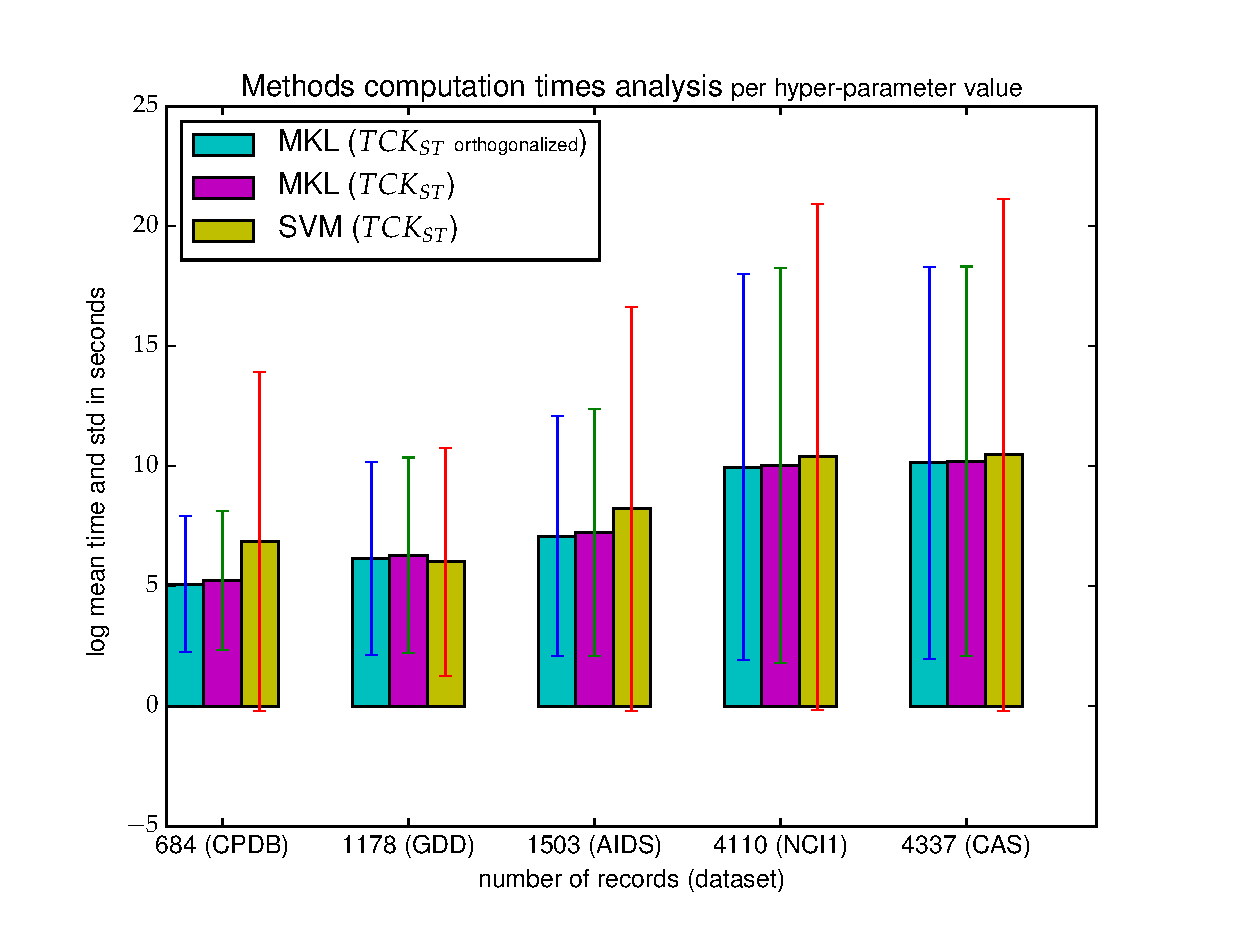
\includegraphics[scale=0.7]{Figures/method_times_avgstd}
    \caption{(DRAFT: is this plot useful? I think it shows the stableness of the algorithm
        over the whole computation and the fact that it is scarcely affected by the hyperparameter; missing data has been plotted at 0.)
        This plot shows the mean computation times among all the hyperparameter values,
        for each learning method and on all the benchmark datasets.
        Each point has the standard deviation among the same set of values plotted as well.
        (DRAFT: I'm not convinced on the presentation, I offset the three lines to highlight the
        standard deviation for each point but I think it could be confusing)
    }
        \label{fig:meantimes}
\end{figure}

\subsection{Analysis of the models performances}

Here we present the empirical results we got from the devised experiments described
in the previous sections.
Data is divided in three tables, one for each of the three combinations we chose.
Each table reports the ROAUC measure with the standard deviation measured with
a nested 10-fold cross validation. (DRAFT: should we substitute it with a 95\% confindence interval?)
ROAUC was chosen over accuracy to be able to compare the results obtained in \cite{gmkl}.

Looking at Table \ref{table:results_st}, it is immediately evident how the results
obtained by our methodology are always comparable when not even better with respect
to the baselines except in when considering the GDD dataset which, as mentioned in
Section \ref{subsec:time_results} is a rather peculiar case given the smaller dimensions
of the parameters grid considered.
While the results for experiment 2 seem in accordance with the results in \cite{gmkl},
the $TCK_{ST}$ (experiment 3) performs significantly worse with our MKL method than with
the SVM.
(DRAFT: experiments 4 and 6 have unexpected high performancs though.)

Table \ref{table:results_stp} present results in accordance with Table \ref{table:results_st}
beside the case of GDD in which apparently the $ODD_{ST+}$ and the version with
contextual informations are able to outperform the baselines while maintaining
comparable performance when used in combination (experiment 1).

From these results something that we can infer is the scarce improvment gained from
using one kernel and its contextualized version in combination with or without
the orthogonalization of the feature space.
All the obtained results shows that either both kernel fare at the same level or
one of them dominates the combination outcome: section \ref{sec:kca} will cover
more in detail this aspect.

\begin{landscape}
%    \begin{table}[ht]
%        \label{table:times}
%        \caption{(DRAFT) Times}
%    \end{table}

    \begin{table}[ht]\footnotesize
        \centering
        \begin{tabular}{|l|l|r|r|r|r|r|}
            \hline
            n. &method&CAS&NCI1&AIDS&CPDB&GDD\\
            \hline
            1& $MKL~(ODDK_{ST}, TCK_{ST})^*$&&&0.8632 $\pm$ 0.0034&\textbf{0.8632 $\pm$ 0.0038}&0.8528 $\pm$ 0.0022\\
            2& $MKL~(ODDK_{ST})^*$&&&0.8627 $\pm$ 0.0035&\textbf{0.8632 $\pm$  0.0029}&0.8543 $\pm$ 0.0024\\
            3& $MKL~(TCK_{ST})^*$&&&\textbf{0.8634 $\pm$ 0.0034}&0.8625 $\pm$ 0.0032&0.8458 $\pm$ 0.0021\\
            \hline
            4& $MKL~(ODDK_{ST}, TCK_{ST})$&0.8960 $\pm$  0.0012&0.9076 $\pm$ 0.0007&0.8468 $\pm$ 0.0042&0.8517 $\pm$ 0.0034&0.8612 $\pm$ 0.0018\\
            5& $MKL~(ODDK_{ST})$&0.8899 $\pm$ 0.0013&0.8976 $\pm$ 0.0010 &0.8388 $\pm$ 0.0044&0.8401 $\pm$ 0.0033&0.8013 $\pm$ 0.0019\\
            6& $MKL~(TCK_{ST})$&0.8954 $\pm$ 0.0013&0.9095 $\pm$ 0.0006&0.8487 $\pm$ 0.0040&0.8525 $\pm$ 0.0030&0.8617 $\pm$ 0.0022\\
            \hline
             & $MKL~(ODDK_{ST})^{**}$&\textbf{0.9049 $\pm$ 0.0008}&0.9144 $\pm$ 0.0008&0.8515 $\pm$ 0.0031&0.8564 $\pm$ 0.0056&0.8498 $\pm$ 0.0026\\
             & $SVM~(ODDK_{ST})^{**}$&0.8982 $\pm$ 0.0017&0.9069 $\pm$ 0.0010&0.8262 $\pm$ 0.0052&0.8442 $\pm$ 0.0067&0.8473 $\pm$ 0.0038\\
            \hline
            7& $SVM~(TCK_{ST} + ODDK_{ST})$&0.9010 $\pm$ 0.0011&0.9110 $\pm$ 0.0011&0.8323 $\pm$ 0.0065&0.8497 $\pm$ 0.0072&0.8627 $\pm$ 0.0018\\
            8& $SVM~(TCK_{ST})$&0.9006 $\pm$ 0.0013&\textbf{0.9150 $\pm$ 0.0011}&0.8225 $\pm$ 0.0067&0.8422 $\pm$ 0.0080&\textbf{0.8674 $\pm$ 0.0026}\\
            \hline
        \end{tabular}
        \caption{\footnotesize ROAUC results ($\pm$ standard deviation) relative to the combination
            of the $ODD_{ST}$ kernel with the $TCK_{ST}$ kernel. Results are
            obtained from a nested 10-fold cross validation. The first column is
            given as a reference to the experiment description given in Section
            \ref{sec:description}.
            The top part of the table contains the results of the main experiments
            while the bottom part those of the baselines.
            Lines marked with $^*$ refer to kernels whose feature space was split
            according to the technique exposed in \ref{subsec:features}.
            Lines marked with $^{**}$ refer to results obtained in \cite{gmkl}.
        }
        \label{table:results_st}
        \medskip

        \begin{tabular}{|l|l|r|r|r|r|r|}
            \hline
            n. & metodo&CAS&NCI1&AIDS&CPDB&GDD\\
            \hline
            1& $MKL (ODDK_{ST+}, TCK_{ST+})^*$&&&0.8632 $\pm$  0.0034&0.8632 $\pm$  0.0038&0.8528 $\pm$ 0.0022\\
            2& $MKL (ODDK_{ST+})^*$&&&0.8628 $\pm$  0.0036&0.8652 $\pm$ 0.0030&\textbf{0.8720 $\pm$ 0.0021}\\
            3& $MKL (TCK_{ST+})^*$&&&\textbf{0.8649 $\pm$  0.0030}&\textbf{0.8666 $\pm$  0.0038}&0.8711 $\pm$ 0.0018 \\
            \hline
            4& $MKL (ODDK_{ST+}, TCK_{ST+})$&&&0.8468 $\pm$ 0.0042&0.8517 $\pm$ 0.0034&0.8612 $\pm$ 0.0018\\
            5& $MKL (ODDK_{ST+})$&&&0.8489 $\pm$  0.0039&0.8461 $\pm$ 0.0036&0.8178 $\pm$ 0.0022\\
            6& $MKL (TCK_{ST+})$&&&0.8503 $\pm$  0.0038&0.8528 $\pm$ 0.0039&0.8645 $\pm$ 0.0018\\
            7& $SVM (TCK_{ST+} + ODDK_{ST+})$&0.9022 $\pm$ 0.0015 &0.9163 $\pm$ 0.0011&0.8256 $\pm$ 0.0068&0.8521 $\pm$ 0.0038&0.8570 $\pm$ 0.0043\\
            8& $SVM (TCK_{ST+})$&0.9008 $\pm$ 0.0017&0.9165 $\pm$ 0.0013&0.8222 $\pm$ 0.0067&0.8462 $\pm$ 0.0048&0.8588 $\pm$ 0.0028\\
            \hline
        \end{tabular}
        \caption{ROAUC results ($\pm$ standard deviation) relative to the combination
                of the $ODD_{ST+}$ kernel with the $TCK_{ST+}$ kernel. Results are
                obtained from a nested 10-fold cross validation. The nomenclature and
            results disposition is analogue to the one of Table \ref{table:results_st}.}
        \label{table:results_stp}
    \end{table}

%    \begin{table}[ht]
%        \label{table:results_wl}
%        \caption{ROAUC results ($\pm$ standard deviation) relative to the combination
%                of the $WL$ kernel with the $WLC$ kernel. Results are
%                obtained from a nested 10-fold cross validation. The nomenclature and
%            results disposition is analogue to the one of Table \ref{table:results_st}.}
%        \label{table:results_wl}
%    \end{table}
\end{landscape}

\section{Kernels Contribution Analysis}
\label{sec:kca}

\begin{figure}[ht]
    \centering
    \includegraphics[scale=0.7]{Figures/weightdist}
    \caption{(DRAFT: this plot is just an example of the available data for furhter analisys.
        I think we may be mainly interested in the experiments were two kernels are combined
        either with or without bucketization of the feature space.)
        Kernel weight distributions for the $TCK_{ST}$ kernel
    computed according to the full parameters grid, on the NCI1 dataset.
    The $x$ axis shows all the employed kernel matrices indexed by their hyperparameters
    values (ascending values left to right), the $y$ axis the weight values.
    Each plot refers to one run of the nested 10-fold cross-validation routine relative to one
    value for the $\Lambda$ parameter of EasyMKL. Weight values are the means between each of the inner
    cross-validation runs. The vertical lines highlight the kernel with the maximum weight for each value of $\Lambda$.}
        \label{fig:weightdist}
\end{figure}


 % Experiments
% Chapter 5

\chapter{Conclusions and Future Work}
\label{Chapter5}
By combining a large number of kernels, derived from selected graph kernel
learning approaches, into a single learning process we wanted to determine if an
effective and overall performance improvement both in computational times and 
in target prediction was possible.

 % Conclusions and future works

%----------------------------------------------------------------------------------------
%	THESIS CONTENT - APPENDICES
%----------------------------------------------------------------------------------------

\appendix % Cue to tell LaTeX that the following "chapters" are Appendices

% Include the appendices of the thesis as separate files from the Appendices folder
% Uncomment the lines as you write the Appendices

%\chapter{A further baseline}
\label{AppendixA}


\section{Hierarchical MKL}
\label{subsec:hierarchy}
% describe the approach in detail (diagram and explaination)

Here we will give a brief description of another baseline method that was implemented
but not tested due to time constraints.
This baseline aims to determine if dividing the combination process in two steps, i.e.
first combine only the kernel generated from the same function and then combine
the weighed sum, could boost the contribution of the single function w.r.t.
the methodology proposed in this work.
This baseline method is a good candidate to be tested in future work related
to this thesis.

\begin{figure}[h]
    \centering
    \includegraphics[scale=0.45]{Figures/hierarchy}
    \caption{\footnotesize The baseline illustrated. The depicted scenario considers
        a single learning phase, where $M > 1$ kernel functions are combined, each giving
        origin to $N$ kernel matrices, though this number can certainly vary
        from function to function depending on the size of the parameters grid, grouped in $M$ sets (a).
        Each set is trained independently using EasyMKL (Section \ref{subsec:easymkl})
        and then used to compute a weighed sum using the weights returned by EasyMKL (b).
        The sum kernels thus obtained ($S_1,\dots,S_M$) are used in combination to train another model (c).
    }
    \label{fig:hmethod}
\end{figure}

% vim: spell spelllang=en_gb

\chapter{Language and Libraries}
\label{AppendixB}

\section{Language}
\label{sec:language}

\section{Libraries}
\label{sec:libraries}


%----------------------------------------------------------------------------------------
%	BIBLIOGRAPHY
%----------------------------------------------------------------------------------------

\printbibliography[heading=bibintoc]

%----------------------------------------------------------------------------------------

\end{document}  
% vim: spell spelllang=en_gb
